% XeLaTeX can use any Mac OS X font. See the setromanfont command below.
% Input to XeLaTeX is full Unicode, so Unicode characters can be typed directly into the source.

% The next lines tell TeXShop to typeset with xelatex, and to open and save the source with Unicode encoding.

%!TEX TS-program = xelatex
%!TEX encoding = UTF-8 Unicode

\documentclass[UTF8]{ctexart}
\usepackage{geometry}                % See geometry.pdf to learn the layout options. There are lots.
\geometry{letterpaper}                   % ... or a4paper or a5paper or ...
%\geometry{landscape}                % Activate for for rotated page geometry
%\usepackage[parfill]{parskip}    % Activate to begin paragraphs with an empty line rather than an indent
\usepackage{graphicx}
\usepackage{amssymb}
\usepackage{enumerate}
\usepackage{booktabs}
\usepackage{multirow}
\usepackage{float}
% Will Robertson's fontspec.sty can be used to simplify font choices.
% To experiment, open /Applications/Font Book to examine the fonts provided on Mac OS X,
% and change "Hoefler Text" to any of these choices.

\usepackage{fontspec,xltxtra,xunicode}
\defaultfontfeatures{Mapping=tex-text}
\setromanfont[Mapping=tex-text]{Hoefler Text}
\setsansfont[Scale=MatchLowercase,Mapping=tex-text]{Gill Sans}
\setmonofont[Scale=MatchLowercase]{Andale Mono}

\title{\Huge \textbf{软件工程项目文档}  \\
\large ~~~~~~~ ———— “鲜活”社团管理平台
 ~\\ ~\\ ~\\ ~\\ ~\\ ~\\ ~\\ ~\\ ~\\ ~\\ ~\\}
\author{
\large 指导老师:黄杰 \\
\large 1452822 洪嘉勇 \\
\large 1454093 夏陈   \\
\large 1452716 张尹嘉 \\
}
%\date{}                                           % Activate to display a given date or no date

\begin{document}
\maketitle

% For many users, the previous commands will be enough.
% If you want to directly input Unicode, add an Input Menu or Keyboard to the menu bar
% using the International Panel in System Preferences.
% Unicode must be typeset using a font containing the appropriate characters.
% Remove the comment signs below for examples.

% \newfontfamily{\A}{Geeza Pro}
% \newfontfamily{\H}[Scale=0.9]{Lucida Grande}
% \newfontfamily{\J}[Scale=0.85]{Osaka}

% Here are some multilingual Unicode fonts: this is Arabic text: {\A السلام عليكم}, this is Hebrew: {\H שלום},
% and here's some Japanese: {\J 今日は}.

\newpage
\tableofcontents
\newpage

\section{引言}
\subsection{背景}
近年来互联网、物联网等发展迅猛,高校校园在这波潮流中可以说是弄潮儿,很多互联网创新平台都在高校中运行得非常稳健。学校也正利用着这股潮流做着相应的改变,校园的管理系统正在渐渐地完善,比如图书馆的预览室已经可以在网上平台预约、校车也可以在网上抢票,但是跟学生们的课余生活最为密切的社团生活似乎并没有纳入学校网络化的考虑范围中。与此同时,我们的社团的活动也开始缺乏新意,社团的团长们缺乏好的点子,而在互联网+的时代下,去创建这样一二个信息共享的渠道是相对容易的,我们渴望在这个时代背景下为同济大学师生创建一个社团管理平台和社团活动信息共享平台,我们将其命名为“鲜活”。
\paragraph{同济大学社团发展现状}
就目前同济大学校园而言,大多数关于社团的操作都非常地繁琐,通信的时间成本和经济成本都非常高,很多社团的发展因为制度问题而变得不健康。体现在以下方面:

\begin{enumerate}[1)]
\item 社团审批需要递交的材料多且审批等待时间长,将导致很多新兴社团痛失很多招生机会
\item 很多社团缺少展示的平台,很多社团因此默默无闻
\item 社团自身没有统一的管理规范,社团管理比较混乱
\item 社团通信流程复杂,通知时间成本高
\item 社团申请场地和申请海报张贴的流程繁琐,等待时间长
\end{enumerate}

\paragraph{线上平台的必要性}
现行的体制使得社团发展受到遏制,一个线上统一管理社团的平台已经成为师生共同的需求。而且传统的在食堂门口发传单等宣传方式早已受到师生们的反感,也为校园环保造成一定的压力,这些事情完全可以放在线上平台上来做。师生们渴望社团是一个又鲜又活的东西,而不是一个抽象的存在,我们需要想办法加强社团的存在感。而这一切都可以通过一个线上的社团管理平台实现。

\paragraph{线上平台的可行性}
在经过背景分析和技术论证之后,我们认为线上平台的可行性很强,具体为以下几点:

\begin{enumerate}[1)]
\item 互联网已经普及
\item 师生群体中智能手机普及率接近100\%
\item 同济大学“同心云”轻应用可以成为一个很好的展示平台
\end{enumerate}

\subsection{假设和约束}
\paragraph{基本假设}本项目需要以一些基本的假定作为项目开展的基础。我们以一些普遍的认识和经验作出以下假设:

\begin{enumerate}[1)]
\item 师生都有手机并可以访问互联网
\item 可以得到学校的支持将平台的展示页面搭载于同济大学“同心云”上
\item 学校可以授权我们得到相关社团和成员的信息
\end{enumerate}

\paragraph{基本约束}
本项目需要以一些基本的约束作为项目开展的基础。我们经过讨论作出以下约束:

\begin{enumerate}[1)]
\item 为减轻服务器访问压力,平台的用户仅限于同济大学的师生,即拥有同济大学学号和工号的人群
\item 团学联老师拥有管理员权限
\item 将尊重所有用户的个人隐私,对用户的个人信息保密
\item 项目开发经费限于大学生国家创新项目经费所给的10000元
\item 项目初期将部署于阿里云服务器上作初步测试
\item 开发时限:2015年-2017年
\item 咨询推送功能将因为课设时间紧迫无法上线
\end{enumerate}

\subsection{用户的特点}
“鲜活”是一个为同济大学师生服务的社团管理和活动信息共享平台,用户主体为同济大学的师生,我们将所有用户罗列如下:

\paragraph{老师}
\subparagraph{概述}
老师是“鲜活”中具有上帝权限的管理员,老师可作为基本用户像学生一样去参加社团甚至可以创建社团,也可以接收到社团的消息推送。但是最关键的是,老师可以审核社团的申请以及社团对场地的申请,只有在老师同意的情况下,社团才可以进行之后的操作。
\subparagraph{具体可执行操作}
老师具体可执行的操作如下:
\newline
\newline
\begin{table}[H]
\centering
\caption{老师}
\begin{tabular}{ccc}
\toprule
操作& 描述\\
\midrule
\textbf{创建社团}& 老师也可以创建属于自己的社团\\
\textbf{加入某个社团}& 老师可以参加某个社团\\
\textbf{参加某个活动}&老师可以参加某个社团的某个活动\\
\textbf{同意社团的创建申请}&老师将审阅所有社团的申请并决定是不是让这个社团成立并入驻“鲜活”\\
\textbf{同意社团的场地申请}&老师将审阅社团的场地申请请求并根据场地借用记录决定是否出借场地\\
\bottomrule
\end{tabular}
\end{table}

\paragraph{社团负责人}
\subparagraph{概述}
社团负责人是“鲜活”中的核心角色,社团负责人在平台中和普通用户一样,只是因为他们申请了社团所以成为了社团负责人这样一个特殊的角色。他们作为社团的核心人物会在平台上管理他们的社团,发布他们的活动和通知,并向上级老师申请活动的场地。
\subparagraph{具体可执行操作}
社团负责人可执行的操作如下:
\newline
\newline
\begin{table}[H]
\centering
\caption{社团负责人}
\begin{tabular}{ccc}
\toprule
操作& 描述\\
\midrule
\textbf{创建社团}& 社团负责人可以向老师发出申请创建属于自己的社团\\
\textbf{加入某个社团}& 社团负责人可以参加某个社团\\
\textbf{参加某个活动}&社团负责人可以参加某个社团的某个活动\\
\textbf{查看社员}&社团负责人可以在“鲜活”中看到谁参加了自己的社团并得到他们的一些信息\\
\textbf{发布活动}&社团负责人可以在“鲜活”中发布自己社团的活动并通过平台向所有社员推送活动信息\\
\textbf{群发短信}& 社团负责人可以根据自己的需求向自己的社员群发短信\\
\textbf{评论}& 社团负责人可以评论不是自己的社团但是他可以评论任何活动\\
\bottomrule
\end{tabular}
\end{table}

\paragraph{普通学生}
\subparagraph{概述}
普通学生是“鲜活”中最基本的也是最多的用户,但即便是这样,一旦等他准备好发起了创建社团的申请并通过审核,就会成为一名社团负责人。普通学生可以加入任何社团中并参加任何社团开始的社团活动,在进入社团后可以下载社团中的资源文件。他们会接收到社团发送的通知。
\subparagraph{具体可执行操作}
普通学生可执行的操作如下:
\newline
\newline
\begin{table}[H]
\centering
\caption{普通学生}
\begin{tabular}{ccc}
\toprule
操作& 描述\\
\midrule
\textbf{创建社团}& 普通学生也可以向老师发起申请创建属于自己的社团\\
\textbf{加入某个社团}& 普通学生可以参加某个社团\\
\textbf{参加某个活动}& 普通学生可以参加某个社团的某个活动\\
\textbf{评论}& 普通学生可以评论任何社团或者任何活动\\
\bottomrule
\end{tabular}
\end{table}

\section{功能需求}
\subsection{系统范围}
\subsubsection{系统开发的意图}
旨在开发一个为同济大学师生服务的线上社团管理平台和社团活动共享平台,将社团从创建到招新到发布活动一体化。
\subsubsection{应用目标}
本系统的应用目标主要为同济大学“同心云”的轻应用和一个web端。
\paragraph{“同心云”轻应用}
本系统将在“同心云”上搭载一个轻应用与服务器相连,用户可以在同心云上查看社团的相关信息并可以进行相关操作,操作将会被同步到web端。但在轻应用上,将不具备社团负责人管理社团的功能,涉及社团更高级的操作将只能在web端登陆之后才可以操作。
\paragraph{web端}
web端将是本系统的重点,在web端我们将开放所有版块的功能,而不仅仅是轻应用上的查看和简单操作。社团负责人可以通过web端操作社团,老师可以通过web端审核各种申请。

\subsubsection{作用范围}
本系统的作用范围为同济大学校内一切拥有同济大学统一认证学号的学生和工号的老师。
\subsection{系统体系结构}
夏
\subsection{系统总体流程}
张
\subsection{需求分析}
夏
\subsubsection{功能建模}
\paragraph{用例规约}
\subparagraph*{场景一}
创建社团
\newline
\begin{figure}[H]
\centering
\includegraphics[width = 0.7\textwidth]{uc-createclub.png}
\end{figure}

\begin{table}[H]
\centering
\caption{创建社团}
\begin{tabular}{|c|c|}
\hline
类别 & 内容 \\
\hline
参与者 & Club Leader, Scrutinize Servic \\
\hline
用例说明 & 用例主要功能是提交创建俱乐部的申请,其实与学生提起申请请求\\
\hline
\multirow{3}*{前置条件}
& 该用户是已经注册过的在校大学生\\
& 该俱乐部名称未被申请过\\
& 提交者已经将必须资料填完整\\
\hline
\multirow{4}*{基本事件}
& 学生在线填写申请材料\\
& 系统将消息放入待提交队列,等待上传\\
& 申请被上传至审核服务\\
& 审核服务将审核分配至管理老师\\
\hline
其他事件 & 无 \\
\multirow{3}*{异常事件}
& 资料提交不完整\\
& 消息添加失败\\
& 审核添加失败\\
\hline
\multirow{2}*{后置条件}
& 审核提交成功,收到短信\\
& 管理老师收到审核消息,放在待处理日志中\\
\hline
\end{tabular}
\end{table}

\subparagraph*{场景二}
下载资源
\newline
\begin{figure}[H]
\centering
\includegraphics[width = 0.7\textwidth]{uc-download.png}
\end{figure}

\begin{table}[H]
\centering
\caption{下载资源}
\begin{tabular}{|c|c|}
\hline
类别 & 内容 \\
\hline
参与者 & User, Qiniu Service \\
\hline
用例说明 & 用例主要功能是用户下载共享文件资源\\
\hline
\multirow{3}*{前置条件}
& 所下载资源可用\\
& 网络通畅\\
& 用户已经注册\\
\hline
\multirow{4}*{基本事件}
& 用户在线下载资源\\
& 系统请求七牛云文件存储\\
& 七牛审核文件是否存在\\
& 文件成功下载\\
\hline
其他事件 & 用户取消下载 \\
\multirow{3}*{异常事件}
& 网络断开\\
& 文件不存在\\
& 云存储宕机\\
\hline
后置条件 & 用户下载成功,获得资源\\
\hline
\end{tabular}
\end{table}

\subparagraph*{场景三}
上传资源
\newline
\begin{figure}[H]
\centering
\includegraphics[width = 0.7\textwidth]{uc-upload.png}
\end{figure}

\begin{table}[H]
\centering
\caption{上传资源}
\begin{tabular}{|c|c|}
\hline
类别 & 内容 \\
\hline
参与者 & Administrator Teacher, Qiniu Service \\
\hline
用例说明 & 用例主要功能是老师上传资源\\
\hline
\multirow{2}*{前置条件}
& 该用户是已经注册的管理老师\\
& 上传的俱乐部/活动已经存在\\
\hline
\multirow{3}*{基本事件}
& 老师上传文件\\
& 系统异步上传文件至七牛云\\
& 七牛云存储返回是否存储成功\\
\hline
其他事件 & 无 \\
\multirow{2}*{异常事件}
& 网络断开\\
& 云存储宕机\\
\hline
\multirow{2}*{后置条件}
& 上传成功\\
& 发送信息给学生\\
\hline
\end{tabular}
\end{table}

\subparagraph*{场景四}
授权俱乐部创建
\newline
\begin{figure}[H]
\centering
\includegraphics[width = 0.7\textwidth]{uc-authorize.png}
\end{figure}

\begin{table}[H]
\centering
\caption{授权俱乐部创建}
\begin{tabular}{|c|c|}
\hline
类别 & 内容 \\
\hline
参与者 & Administer Teacher, Scrutinize Service \\
\hline
用例说明 & 用例主要功能是初步审核俱乐部,然后上交至审核服务\\
\hline
\multirow{2}*{前置条件}
& 用户已经注册为管理员老师\\
& 学生已经递交了相关申请资料至审核服务\\
\hline
\multirow{3}*{基本事件}
& 管理员老师从审核服务处拿到已经审批过并且资料完整的申请信息\\
& 管理员老师审核该俱乐部的资料\\
& 审核过后再将审核结果递交至审核服务处\\
\hline
其他事件 & 学生取消申请,老师直接将审核置为不通过 \\
\hline
异常事件 & 无\\
\hline
\multirow{3}*{后置条件}
& 审核通过\\
& 审核拒绝\\
& 审核服务返回信息给申请人\\
\hline
\end{tabular}
\end{table}

\subparagraph*{场景五}
社团负责人发布社团信息
\newline
\begin{figure}[H]
\centering
\includegraphics[width = 0.7\textwidth]{uc-sendmessage.png}
\end{figure}

\begin{table}[H]
\centering
\caption{社团负责人发布社团信息}
\begin{tabular}{|c|c|}
\hline
类别 & 内容 \\
\hline
参与者 & Club Leader, Club \\
\hline
用例说明 & 用例主要功能是社团负责人发送社团内部消息\\
\hline
\multirow{2}*{前置条件}
& 用户已经注册为社团负责人\\
& 有需要发布的消息\\
\hline
\multirow{3}*{基本事件}
& 社团负责人发布消息\\
& 系统缓存信息\\
& 消息被发布给各个社团社员\\
\hline
其他事件 & 学生取消申请,老师直接将审核置为不通过 \\
\hline
\multirow{2}*{异常事件}
& 部分成员未收到信息\\
& 缓存溢出\\
\hline
\multirow{1}*{后置条件}
& 社团成员收到信息\\
\hline
\end{tabular}
\end{table}

\subparagraph*{场景六}
社团负责人发布活动信息
\newline
\begin{figure}[H]
\centering
\includegraphics[width = 0.7\textwidth]{uc-sendactivity-message.png}
\end{figure}

\begin{table}[H]
\centering
\caption{社团负责人发布活动信息}
\begin{tabular}{|c|c|}
\hline
类别 & 内容 \\
\hline
参与者 & Club Leader, Activity \\
\hline
用例说明 & 用例主要功能是社团负责人发送社团举办活动消息\\
\hline
\multirow{3}*{前置条件}
& 用户已经注册为社团负责人\\
& 活动已经注册并存在\\
& 有需要发布的活动信息\\
\hline
\multirow{3}*{基本事件}
& 社团负责人发布消息\\
& 系统缓存信息\\
& 消息被发布给各个社团社员\\
\hline
其他事件 & 无 \\
\hline
\multirow{2}*{异常事件}
& 部分参加互动成员未收到信息\\
& 缓存溢出\\
\hline
\multirow{1}*{后置条件}
& 社团成员收到信息\\
\hline
\end{tabular}
\end{table}

\subparagraph*{场景七}
学生申请加入社团
\newline
\begin{figure}[H]
\centering
\includegraphics[width = 0.7\textwidth]{uc-applyforclub.png}
\end{figure}

\begin{table}[H]
\centering
\caption{学生申请加入社团}
\begin{tabular}{|c|c|}
\hline
类别 & 内容 \\
\hline
参与者 & Student ,Club ,ScrutinizeServices \\
\hline
用例说明 & 用例主要功能是向系统递交申请信息,审核服务进行审核\\
\hline
\multirow{1}*{前置事件}
& 该用户尚未加入所申请的俱乐部\\
\hline
\multirow{4}*{基本事件}
& 学生向准备注册进入某一俱乐部,成为其中一员\\
& 学生提交必要的申请资料\\
& 系统接收申请后递交往审查服务 \\
& 审查服务放进待审查队列\\
\hline
其他事件 & 无 \\
\hline
\multirow{2}*{异常事件}
& 用户已经是该俱乐部成员\\
& 用户资料不完整\\
\hline
\multirow{1}*{后置条件}
& 审查服务递送申请给社团负责人\\
\hline
\end{tabular}
\end{table}

\subparagraph*{场景八}
用户注册活动
\newline
\begin{figure}[H]
\centering
\includegraphics[width = 0.7\textwidth]{uc-registeractivity.png}
\end{figure}

\begin{table}[H]
\centering
\caption{学生申请注册活动}
\begin{tabular}{|c|c|}
\hline
类别 & 内容 \\
\hline
参与者 & User \\
\hline
用例说明 & 用例主要功能是用户注册活动\\
\hline
\multirow{2}*{前置事件}
& 活动已经注册并存在\\
& 活动人数未到上限\\
\hline
\multirow{2}*{基本事件}
& 用户注册活动\\
& 系统校验相关信息后,自动安排\\
\hline
其他事件 & 无 \\
\hline
\multirow{1}*{异常事件}
& 活动被取消\\
\hline
\multirow{1}*{后置条件}
& 用户注册活动成功\\
\hline
\end{tabular}
\end{table}

\subparagraph*{场景九}
用户收到推送信息
\newline
\begin{figure}[H]
\centering
\includegraphics[width = 0.7\textwidth]{uc-getmessage.png}
\end{figure}

\begin{table}[H]
\centering
\caption{用户收到推送信息}
\begin{tabular}{|c|c|}
\hline
类别 & 内容 \\
\hline
参与者 & User \\
\hline
用例说明 & 用例主要功能是用户接受推送信息\\
\hline
\multirow{1}*{前置事件}
& 用户注册并启用推送功能\\
\hline
\multirow{2}*{基本事件}
& 用户订阅消息\\
& 系统根据用户点击习惯进行推送\\
\hline
其他事件 & 无 \\
\hline
\multirow{1}*{异常事件}
& 用户关闭推送功能\\
\hline
\multirow{1}*{后置条件}
& 用户得到推送信息\\
\hline
\end{tabular}
\end{table}

\subparagraph*{场景十}
管理员老师审核
\newline
\begin{figure}[H]
\centering
\includegraphics[width = 0.7\textwidth]{uc-admin.png}
\end{figure}

\begin{table}[H]
\centering
\caption{管理员老师审核}
\begin{tabular}{|c|c|}
\hline
类别 & 内容 \\
\hline
参与者 & Administrator \\
\hline
用例说明 & 用例主要功能是管理员老师对信息进行审核\\
\hline
\multirow{2}*{前置事件}
& 管理员老师已经注册\\
& 有待审核的项目\\
\hline
\multirow{3}*{基本事件}
& 系统将待审核项目推送至老师管理平台\\
& 老师逐项审核,向系统发送审核结果以及描述\\
& 系统将审核信息推送至请求申请的人\\
\hline
其他事件 & 无 \\
\hline
\multirow{1}*{异常事件}
& 审核事件过期\\
\hline
\multirow{1}*{后置条件}
& 将审核结果发布回申请者那里\\
\hline
\end{tabular}
\end{table}

\subparagraph*{场景十一}
短信提醒功能
\newline
\begin{figure}[H]
\centering
\includegraphics[width = 0.7\textwidth]{uc-alidayu.png}
\end{figure}

\begin{table}[H]
\centering
\caption{短信提醒功能}
\begin{tabular}{|c|c|}
\hline
类别 & 内容 \\
\hline
参与者 & User, Text Service \\
\hline
用例说明 & 用例主要功能是注册活动后用户会收到短信提醒\\
\hline
\multirow{1}*{前置事件}
& 用户在注册时填写了正确的手机号码\\
\hline
\multirow{2}*{基本事件}
& 用户注册活动并成功录入\\
& 系统将注册成功的信息通过阿里大于推送至用户手机\\
\hline
其他事件 & 无 \\
\hline
\multirow{2}*{异常事件}
& 短信遭到拦截\\
& 手机号有误\\
\hline
\multirow{1}*{后置条件}
& 用户收到提醒短信\\
\hline
\end{tabular}
\end{table}

\paragraph{数据流图}
以下将分为资源上传图、审核服务数据流图和推荐系统数据流图三个版块来介绍该系统的数据流图
\subparagraph*{资源上传流图}
以下为资源上传流图:\\
\begin{figure}[H]
\centering
\includegraphics[width = 0.9\textwidth]{upload-df.png}
\end{figure}

\textbf{顶层}:老师和同学通过平台可以上传和下载资源,做到资源共享

\textbf{0层}:\\
\begin{figure}[H]
\centering
\includegraphics[width = 0.9\textwidth]{upload0-df.png}
\end{figure}
简介:\\
\emph{第一层~Resources classification}:学生和老师的资源上传后首先会被分类,区分的标准为文件格式,并将分了的中间过程记录如日志。\\
\emph{第二层~Resources filtration}:将资源进行过滤,这一步主要是对资源进行审查,审查完成后将文件导入七牛云文件系统并记录资源信息到数据库。\\

\textbf{1层}:\\
\begin{figure}[H]
\centering
\includegraphics[width = 0.9\textwidth]{upload1-df.png}
\end{figure}
简介:\\
\emph{第一层~Fetch resources}:资源来源为学生和老师上传的资源,并将获取信息存入到日志。\\
\emph{第二层~Make tags}:为资源打上分类的标签,并将分类信息存入日志中。\\
\emph{第三层~Concat resources}:将资源整合起来,并向下传递。\\

\textbf{3层}:\\
\begin{figure}[H]
\centering
\includegraphics[width = 0.9\textwidth]{upload2-df.png}
\end{figure}
简介:\\
\emph{第一层~Check the completion}:根据日志信息检查文件的完整性。\\
\emph{第二层~Combine resources by tags}:将数据按照标签整合起来,完成分类。\\

\subparagraph*{审核服务数据流图}
以下为审核服务数据流图:\\
\begin{figure}[H]
\centering
\includegraphics[width = 0.9\textwidth]{download-df.png}
\end{figure}

\textbf{顶层}:学生递交申请通过鲜活平台交由老师审核,然后老师批阅后在将信息通过鲜活发布到学生手里。\\

\textbf{0层}:\\
\begin{figure}[H]
\centering
\includegraphics[width = 0.9\textwidth]{download0-df.png}
\end{figure}
简介:\\
\emph{第一层~Check the completion of the submission}:首先检查递送的申请资料是否完整。\\
\emph{第二层~Buffer the application}:将申请信息放入申请队列,成为待处理的申请,同时将申请信息添加进数据库,将申请资料存储到七牛云上。\\
\emph{第三层~Scrutinized by teacher}:将申请递送至老师客户端进行审查,并接受审核决定。\\
\emph{第四层~Decision Format}:将决定格式化后处理为读者友好型的信息。\\

\textbf{1层}:\\
\begin{figure}[H]
\centering
\includegraphics[width = 0.9\textwidth]{download1-df.png}
\end{figure}
简介:\\
\emph{第一层~format check}:学生申请递送后,先查看格式填写是否正确。\\
\emph{第二层~proof check}:将递送后的信息进行核对,确保正确。\\
\emph{第三层~identity check}:对学生信息进行核对,然后将申请记录下来。\\

\textbf{2层}:\\
\begin{figure}[H]
\centering
\includegraphics[width = 0.9\textwidth]{download2-df.png}
\end{figure}
简介:\\
\emph{第一层~List the applications}:在老师客户端上列出所有待审核的申请信息,审核内容来源是申请队列和相对应的递交资料,然后将学生申请记录下来。
\\
\emph{第二层~Async wait}:异步等待决策信息。\\

\subparagraph*{推荐系统数据流图}
以下为推荐系统数据流图:\\
\begin{figure}[H]
\centering
\includegraphics[width = 0.9\textwidth]{recommend-df.png}
\end{figure}

\textbf{顶层}:推荐系统的输入来源于用户,用户的平时点击,收藏和爱好等因素都会作为推荐系统的输入特征来为推荐系统诸如数据来源,输出给用户为推荐数据,通过数据传输显示在用户的页面上。\\

\textbf{0层}:\\
\begin{figure}[H]
\centering
\includegraphics[width = 0.9\textwidth]{recommend0-df.png}
\end{figure}
简介:扩充了推荐系统,更加具体的展现了推荐系统的抽象流程,从用户界面得到的数据,模式的评估,数据挖掘引擎和数据仓库的存储模块,构建了完整的推荐系统逻辑。\\

\textbf{1层}:\\
\begin{figure}[H]
\centering
\includegraphics[width = 0.6\textwidth]{recommend1-df.png}
\end{figure}
简介:扩充了Graphical User Interface。\\
\emph{第一层~fajax,post传送数据}:将用户的点击作为数据流以json格式传送的后端,ajax传送是因为以下几点:\\
\begin{enumerate}[1)]
\item 因为能在不刷新整个页面的前提下与服务器通信维护数据。这使得Web应用程序更为迅捷地响应用户交互,并避免了在网络上发送那些没有改变的信息,减少用户等待时间,带来非常好的用户体验
\item 看数据。这里包含两个部分:一是看元数据,包括字段解释、数据来源、代码表等等一切描述数据的信息;二是抽取一部分数据,使用人工查看方式,对数据本身有一个直观的了解,并且初步发现一些问题,为之后的处理准备。
\end{enumerate}
具体步骤:\\
\begin{enumerate}[1)]
\item 因为能在不刷新整个页面的前提下与服务器通信维护数据。这使得Web应用程序更为迅捷地响应用户交互,并避免了在网络上发送那些没有改变的信息,减少用户等待时间,带来非常好的用户体验
\item 看数据。这里包含两个部分:一是看元数据,包括字段解释、数据来源、代码表等等一切描述数据的信息;二是抽取一部分数据,使用人工查看方式,对数据本身有一个直观的了解,并且初步发现一些问题,为之后的处理准备。
\end{enumerate}

\emph{第二层~data cleaning,即数据清洗}:将递送后的信息进行核对,确保正确。\\
\begin{figure}[H]
\centering
\includegraphics[width = 0.9\textwidth]{data-cleaning-df.png}
\end{figure}
数据清洗主要是为了解决以下两点:\\
\begin{enumerate}[1)]
\item 将数据导入处理工具。通常来说,建议使用数据库,单机跑数搭建MySQL环境即可。如果数据量大(千万级以上),可以使用文本文件存储+Python操作的方式。
\item 使用异步方式与服务器通信,不需要打断用户的操作,具有更加迅速的响应能力。优化了Browser和Server之间的沟通,减少不必要的数据传输、时间及降低网络上数据流量
\item 可以把以前一些服务器负担的工作转嫁到客户端,利用客户端闲置的能力来处理,减轻服务器和带宽的负担,节约空间和宽带租用成本。并且减轻服务器的负担,AJAX的原则是“按需取数据”,可以最大程度的减少冗余请求和响应对服务器造成的负担,提升站点性能
\item 基于标准化的并被广泛支持的技术,不需要下载浏览器插件或者小程序,但需要客户允许JavaScript在浏览器上执行。随着Ajax的成熟,一些简化Ajax使用方法的程序库也相继问世。同样,也出现了另一种辅助程序设计的技术,为那些不支持JavaScript的用户提供替代功能
\item WEB中的界面与应用分离(也可以说是数据与呈现分离),有利于分工合作、减少非技术人员对页面的修改造成的WEB应用程序错误、提高效率、也更加适用于现在的发布系统
\end{enumerate}
具体步骤:\\
\begin{enumerate}[1)]
\item 缺失值是最常见的数据问题,处理缺失值也有很多方法,我建议按照以下四个步骤进行:\\
1、	确定缺失值范围:对每个字段都计算其缺失值比例,然后按照缺失比例和字段重要性,分别制定策略。\\
2、	去除不需要的字段,直接删掉即可。建议清洗每做一步都备份一下,或者在小规模数据上试验成功再处理全量数据,不然删除错了会追悔莫及。\\
3、填充缺失内容:某些缺失值可以进行填充,可以统计比例,也可以用机器学习算法填充。
\item 格式内容清洗:\\
1、	时间、日期、数值、全半角等显示格式不一致\\
2、	内容中有不该存在的字符
\item 逻辑错误清洗:\\
1、	去重\\
2、	去除不合理值\\
3、修正矛盾内容
\item 非需求数据清洗
\item 关联性验证
\end{enumerate}
\emph{第三层~data integration,即数据整合}:数据整合使用的工具为Pentaho,作为ETL脚本的支撑,采用mapreduce作为数据流的整合和进一步格式化。\\
\emph{第四层~data transformation,即数据转化}:Hive 集群将分布式数据库的表导出为csv文件格式。\\

\textbf{2层}:\\
\begin{figure}[H]
\centering
\includegraphics[width = 0.9\textwidth]{recommend2-df.png}
\end{figure}
简介:\\
\emph{第一层~将csv格式读为数据DataFrame格式}:由于DataFrame超强的处理性能,在处理数据的时候可以很轻松的读取大规模数据,并且使得程序员可以用操纵excel表格的方式做代码处理。\\
\emph{第二层~管道化的方式对即将进入model训练的数据做进一步处理}:Pipeline架构允许流水线处理。流水线上除最后一个工作以外,其他都要执行fit\_transform方法,且上一个工作输出作为下一个工作的输入。\\
\emph{第三层~模型选择}:为了使得训练数据达到一定精度,用不同的机器学习模型对数据进行训练,并则优选取。\\
\emph{第四层~模型优化}:对最终选择出来的模型进行模型参数的调优得到最终的优化模型。\\

\textbf{3层}:\\
\begin{figure}[H]
\centering
\includegraphics[width = 0.9\textwidth]{recommend3-df.png}
\end{figure}
简介:\\
\emph{第一层~tensorflow frame}:数据流入tensorflow,根据配置进行cpu和gpu的自动分配。\\
\emph{第二层~tensorflow cnn model}:将测试数据放入卷积神经网络,完成tensorflow对于数据的配置。\\
\emph{第三层~training data}:将数据分为测试数据和训练数据,对文本进行分类。\\
\emph{第四层~testing and validating data}:将数据进行交叉验证和精确度检验。\\
\emph{第五层~data schematized}:最后做数据的模型化,预备导入分布式数据库。\\

\textbf{4层}:\\
\begin{figure}[H]
\centering
\includegraphics[width = 0.9\textwidth]{recommend4-df.png}
\end{figure}
简介:\\
\emph{第一层~hive insertion}:将训练结果插入分布式数据库\\
\emph{第二层~metadata storage}:将日志和hive数据的信息存入元数据库。\\
\emph{第三层~master}:由master节点分布存储任务。\\
\emph{第四层~slave store data}:Slave节点将数据存入分布式文件系统。\\
\emph{第五层~Message deliver}:将推送信息向上层传递。\\

\paragraph{活动图}
以下是上传文件、申请活动、推荐系统的活动图:
\subparagraph*{学生上传文件活动图}
如下:\\
\begin{figure}[H]
\centering
\includegraphics[width = 0.9\textwidth]{upload-ac.png}
\end{figure}

\subparagraph*{申请活动图}
如下:\\
\begin{figure}[H]
\centering
\includegraphics[width = 0.9\textwidth]{apply-ac.png}
\end{figure}

\subparagraph*{推荐系统活动图}
如下:\\
\begin{figure}[H]
\centering
\includegraphics[width = 0.6\textwidth]{recommend-ac.png}
\end{figure}


\subsubsection{数据建模}
本系统的数据模型主要概括为:实体类(Entity)、仓库类(Repository)、服务类(Service)和控制器类(Controller),本节将着重介绍实体类、仓库类和服务类,控制器类所构成的模型在数据流图中会更加形象,故在本节中略去。
以下为本系统的数据包图和全部类的汇总:
\newline
\newline
\begin{figure}
\centering
\includegraphics[width = 0.7\textwidth]{package.png}
\end{figure}

\begin{table}[H]
\centering
\caption{类汇总}
\begin{tabular}{|c|c|c|}
\hline
\multicolumn{3}{|c|}{汇总}\\
\hline
类别& 类名& 备注\\
\hline
\multirow{7}*{实体类(Entity)}
&Student& 学生\\
&Teacher&老师\\
&Club&社团\\
&Activity&活动\\
&Apply&申请\\
&Comment&评论\\
&ClubFile&社团资源文件\\
\hline
\multirow{7}*{仓库类(repository)}
&StudentRepository&学生库\\
&TeacherRepository&老师库\\
&ClubRepository&社团库\\
&ActivityRepository&活动库\\
&ApplyRepository&请求库\\
&CommentRepository&评论库\\
&clubFileRepository&社团文件资源库\\
\hline
\multirow{7}*{仓库类(repository)}
&StudentService&学生库接口\\
&TeacherService&老师库接口\\
&ClubService&社团库接口\\
&ActivityService&活动库接口\\
&ApplyService&请求库接口\\
&CommentService&评论库接口\\
&clubFileService&社团文件资源库接口\\
\hline
\end{tabular}
\end{table}

\paragraph{ER关系图}
本系统的数据库ER关系图如下:
\newline
\begin{figure}[H]
\centering
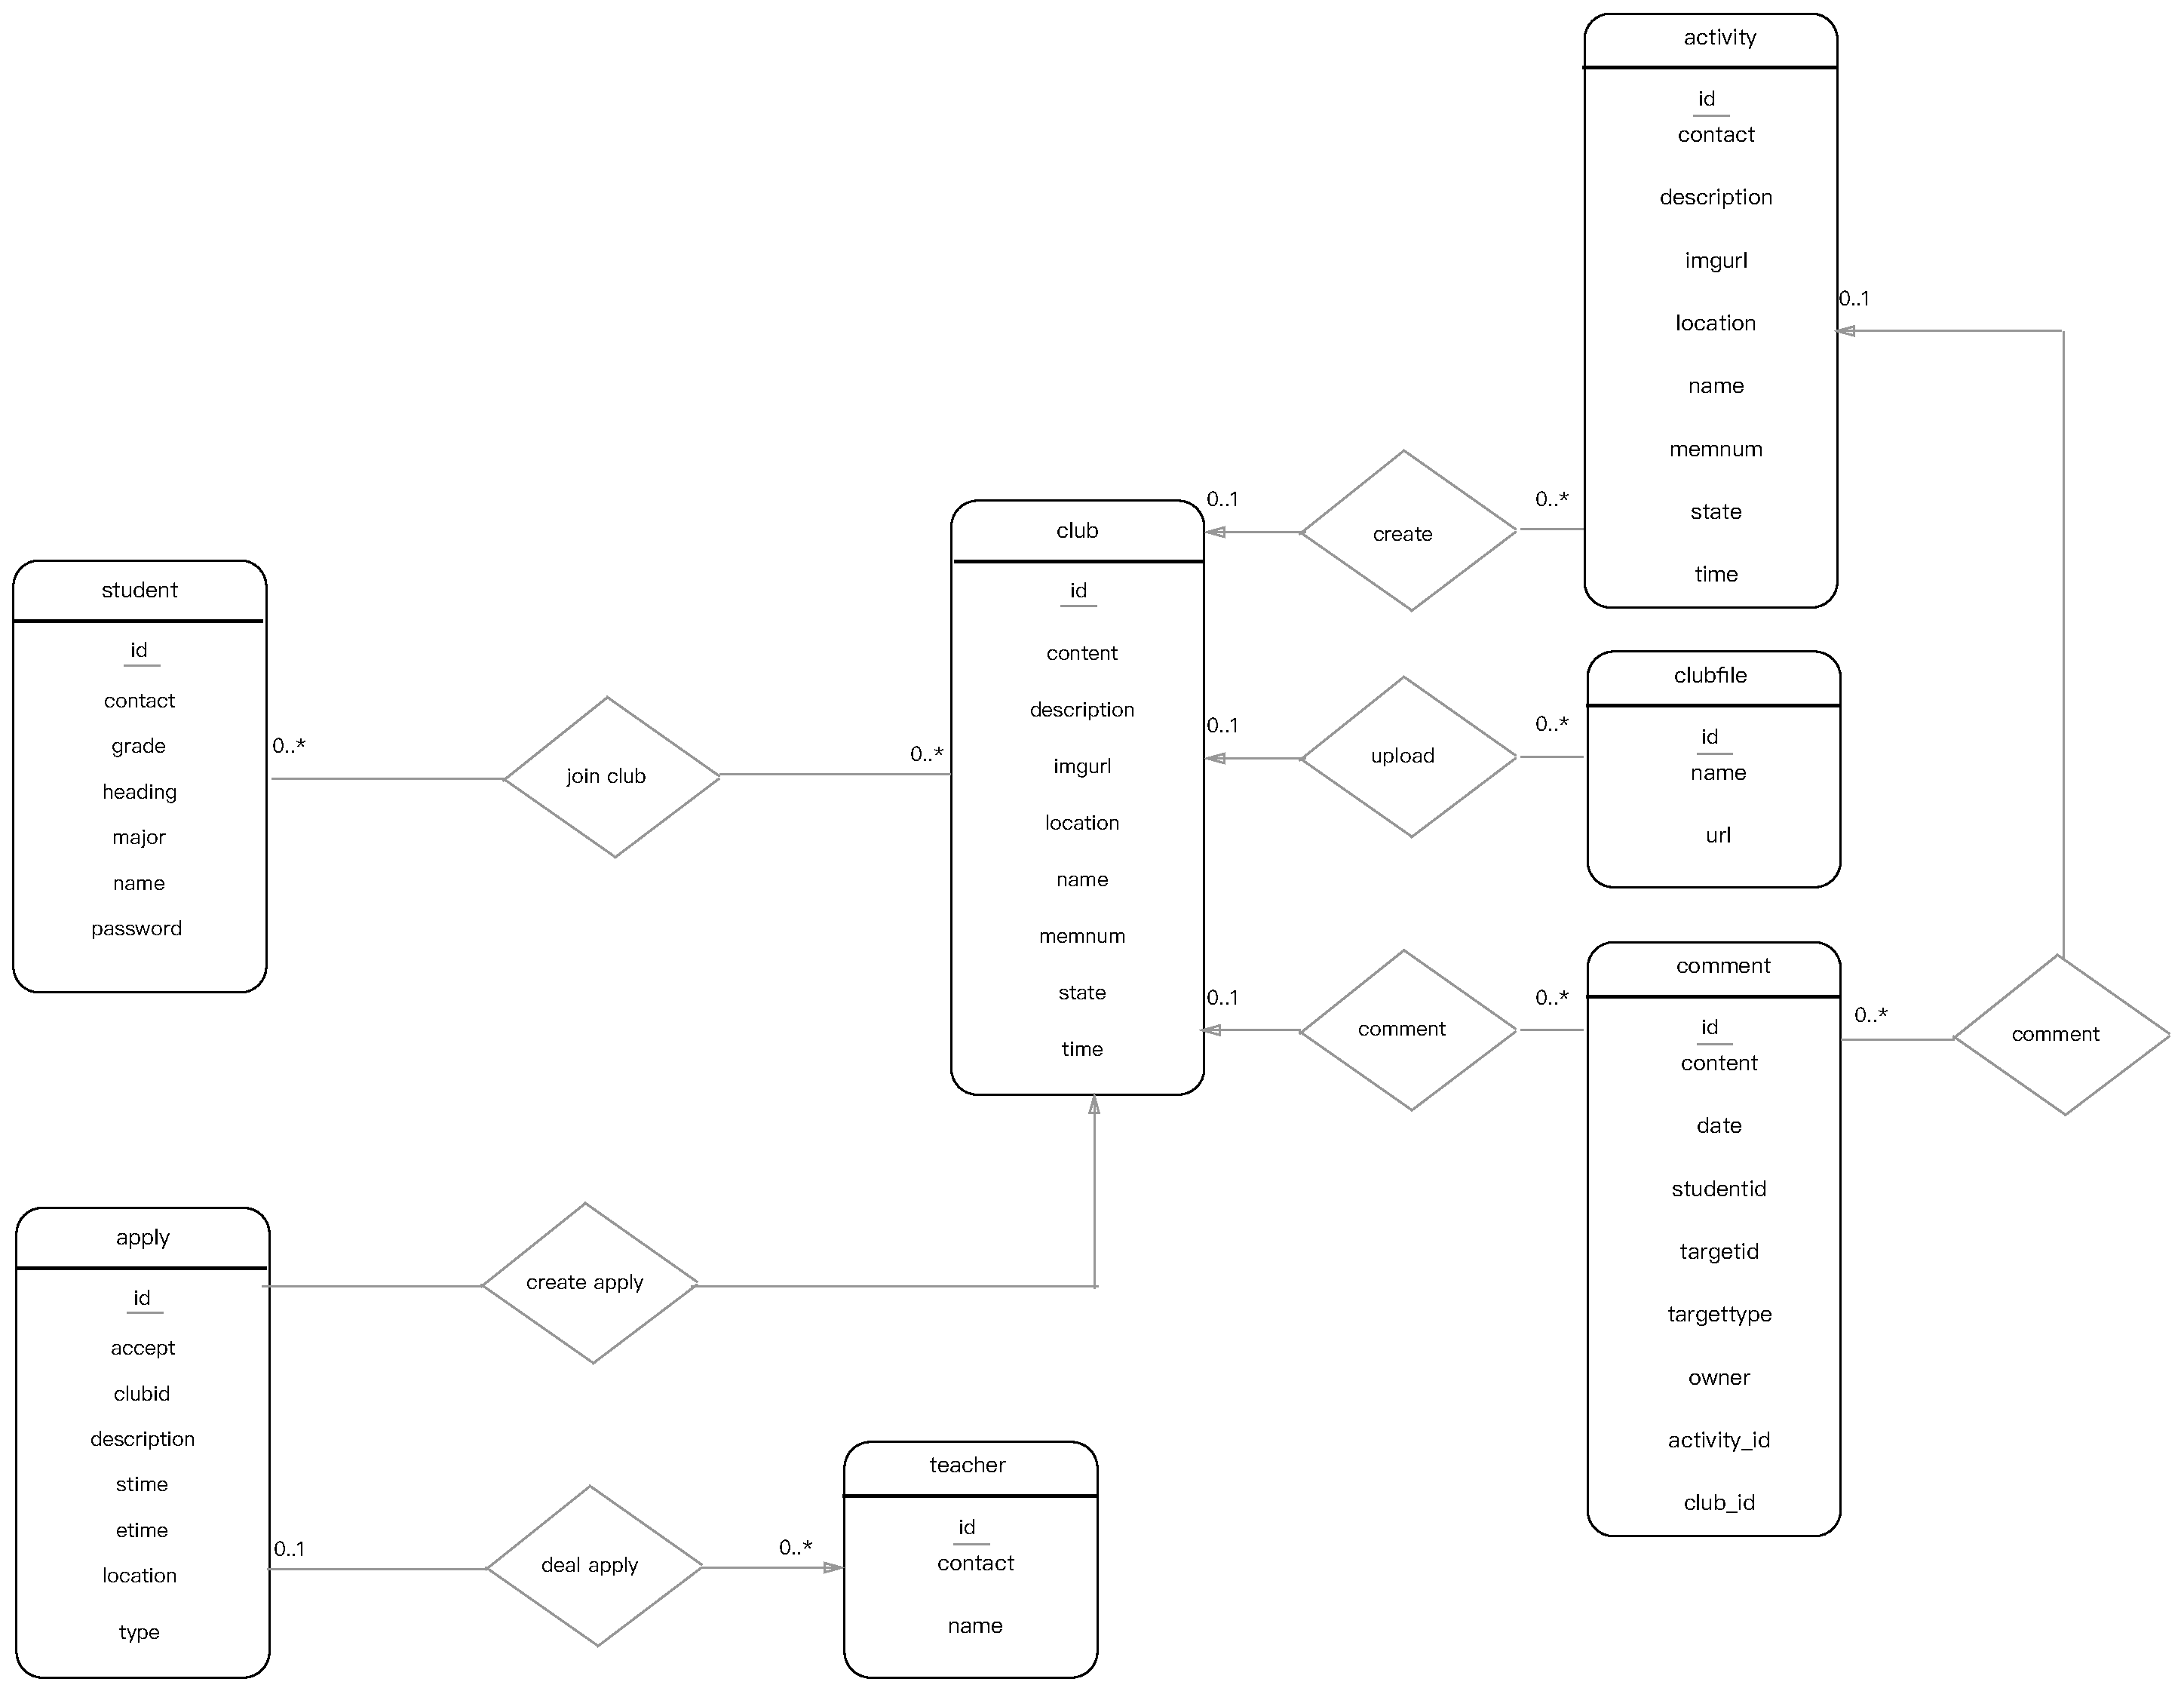
\includegraphics[width = 1.0\textwidth]{er.eps}
\end{figure}

\subparagraph{student \& club}
如下图所示,student和club以join club关系集维系,二者为多对多的关系,student申请加入club之后二者就相互关联
\newline
\begin{figure}[H]
\centering
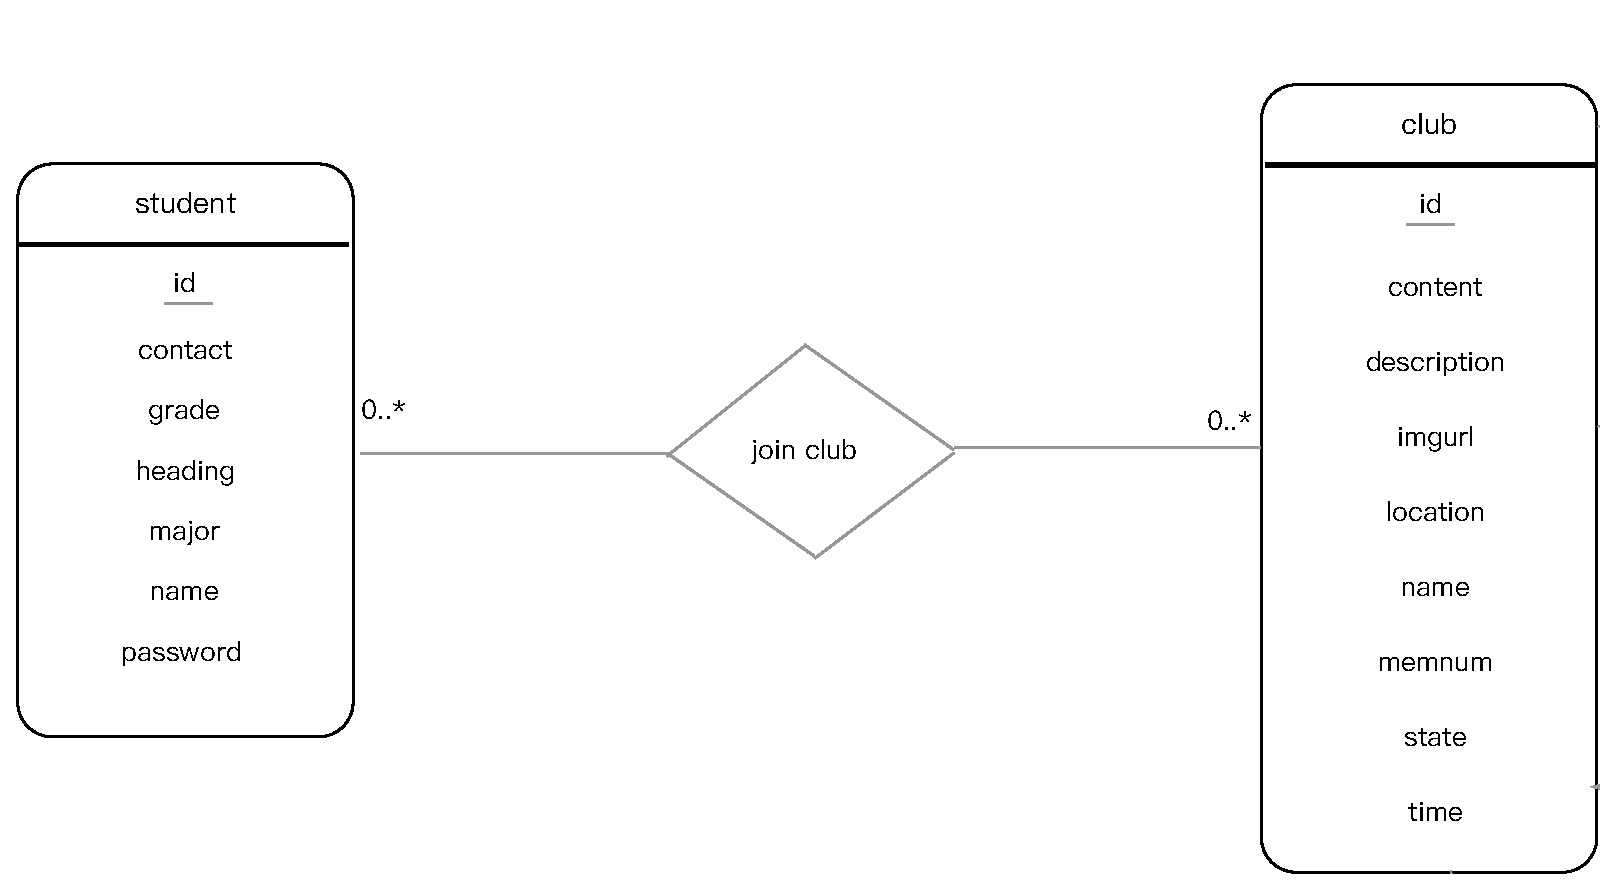
\includegraphics[width = 0.8\textwidth]{student-club-er.eps}
\end{figure}

\subparagraph{club \& activity \& clubFile \& comment}
如下图所示,club跟activity、clubFile、comment向关联。club与activity为一对多的关系,二者以create关系集维系,club可以创建很多个activity;club与clubFile也是一对多的关系,二者以upload关系集相维系,一个club可以拥有多个clubFile;club与comment也为一对多的关系,二者以comment关系集相维系,一个club可以对应多个comment。
\newline
\begin{figure}[H]
\centering
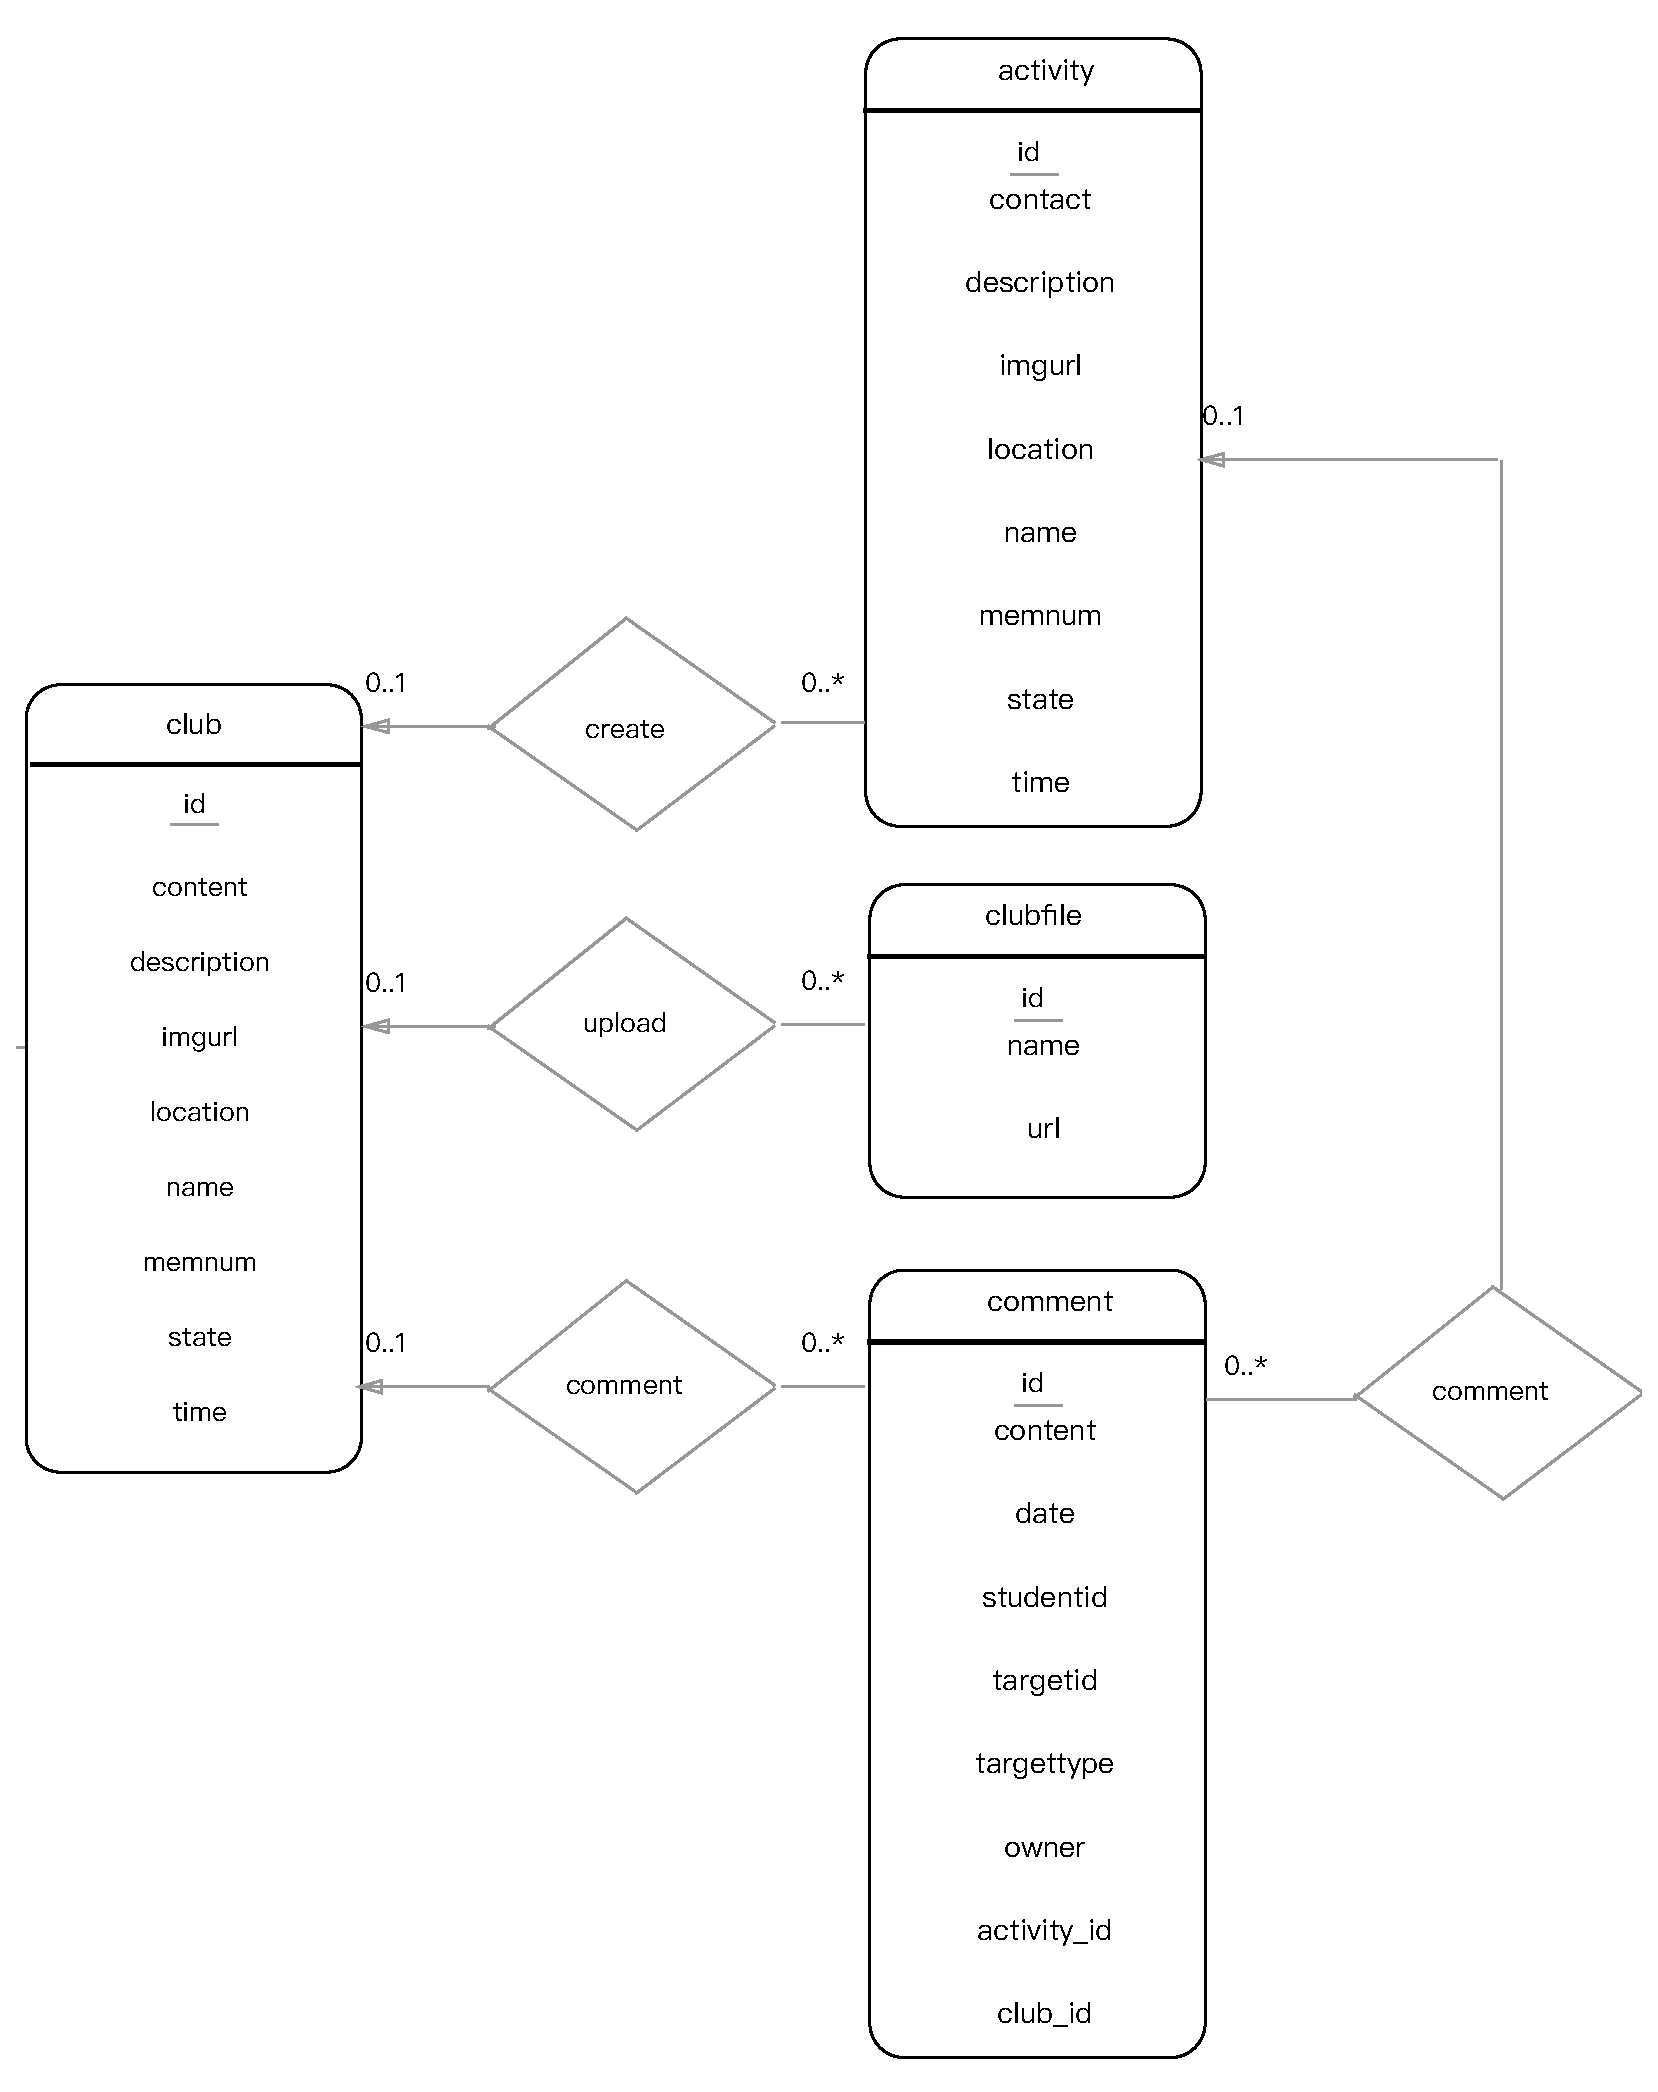
\includegraphics[width = 0.7\textwidth]{club-*-er.eps}
\end{figure}

\subparagraph{comment \& activity}
如下图所示,comment跟activity为一对多的关系,二者以comment关系集相维系,一个activity可以对应有多个comment。
\newline
\begin{figure}[H]
\centering
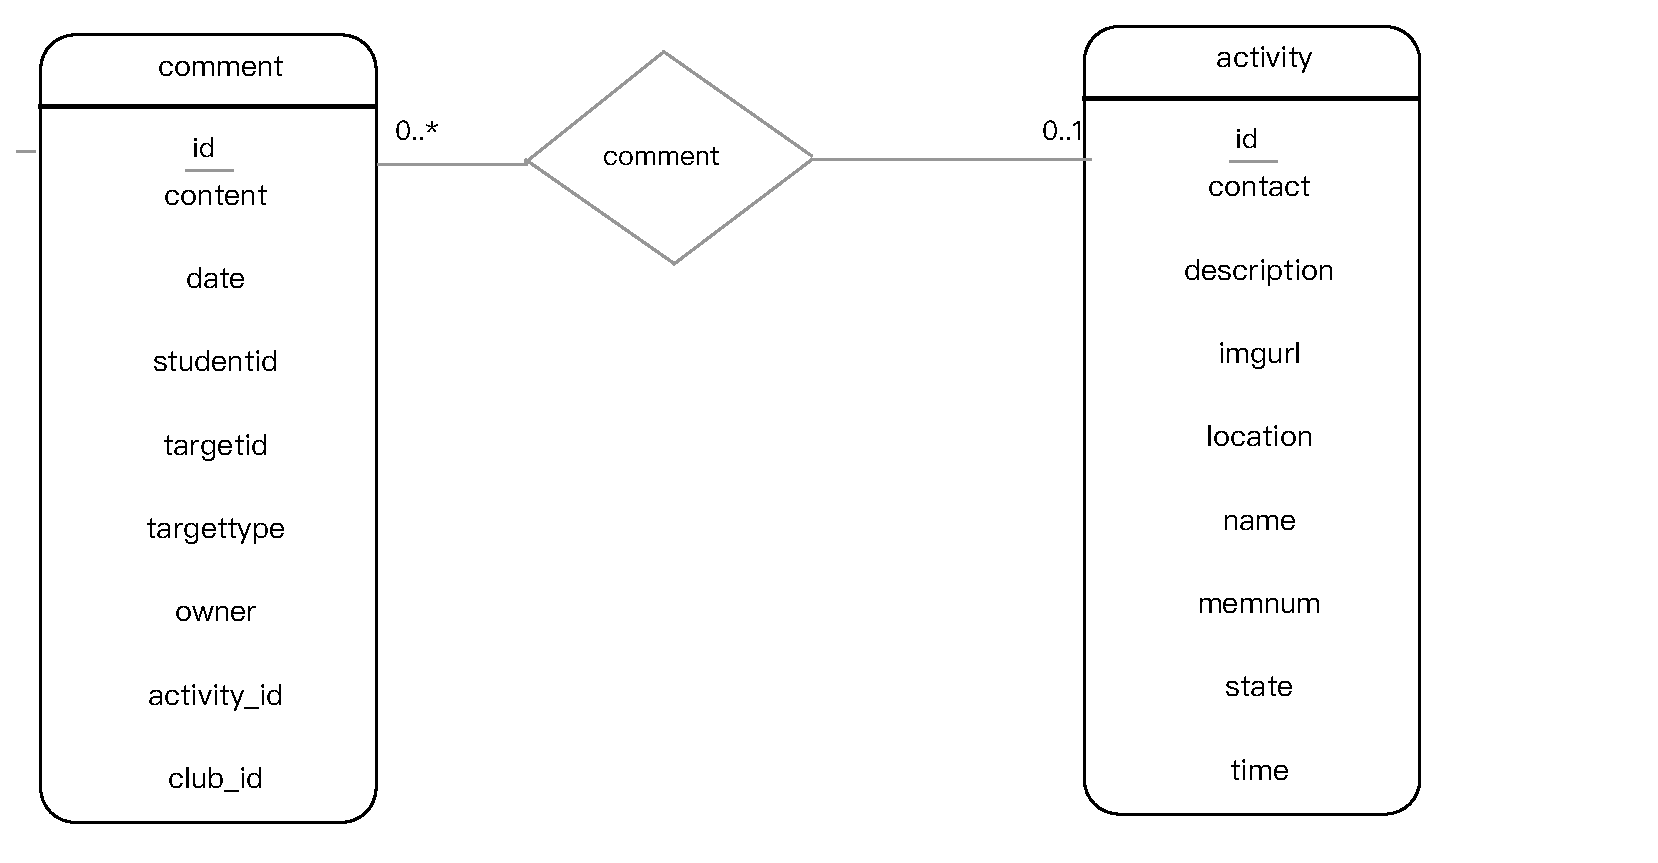
\includegraphics[width = 1.0\textwidth]{activity-comment-er.eps}
\end{figure}

\subparagraph{apply \& club \& teacher}
如下图所示,apply和club、teacher相关联,apply与club为多对一的关系,二者以create apply关系集相维系;apply与teacher为多对一的关系,二者以deal apply关系集相维系,一个teacher可以处理多个apply。
\newline
\begin{figure}[H]
\centering
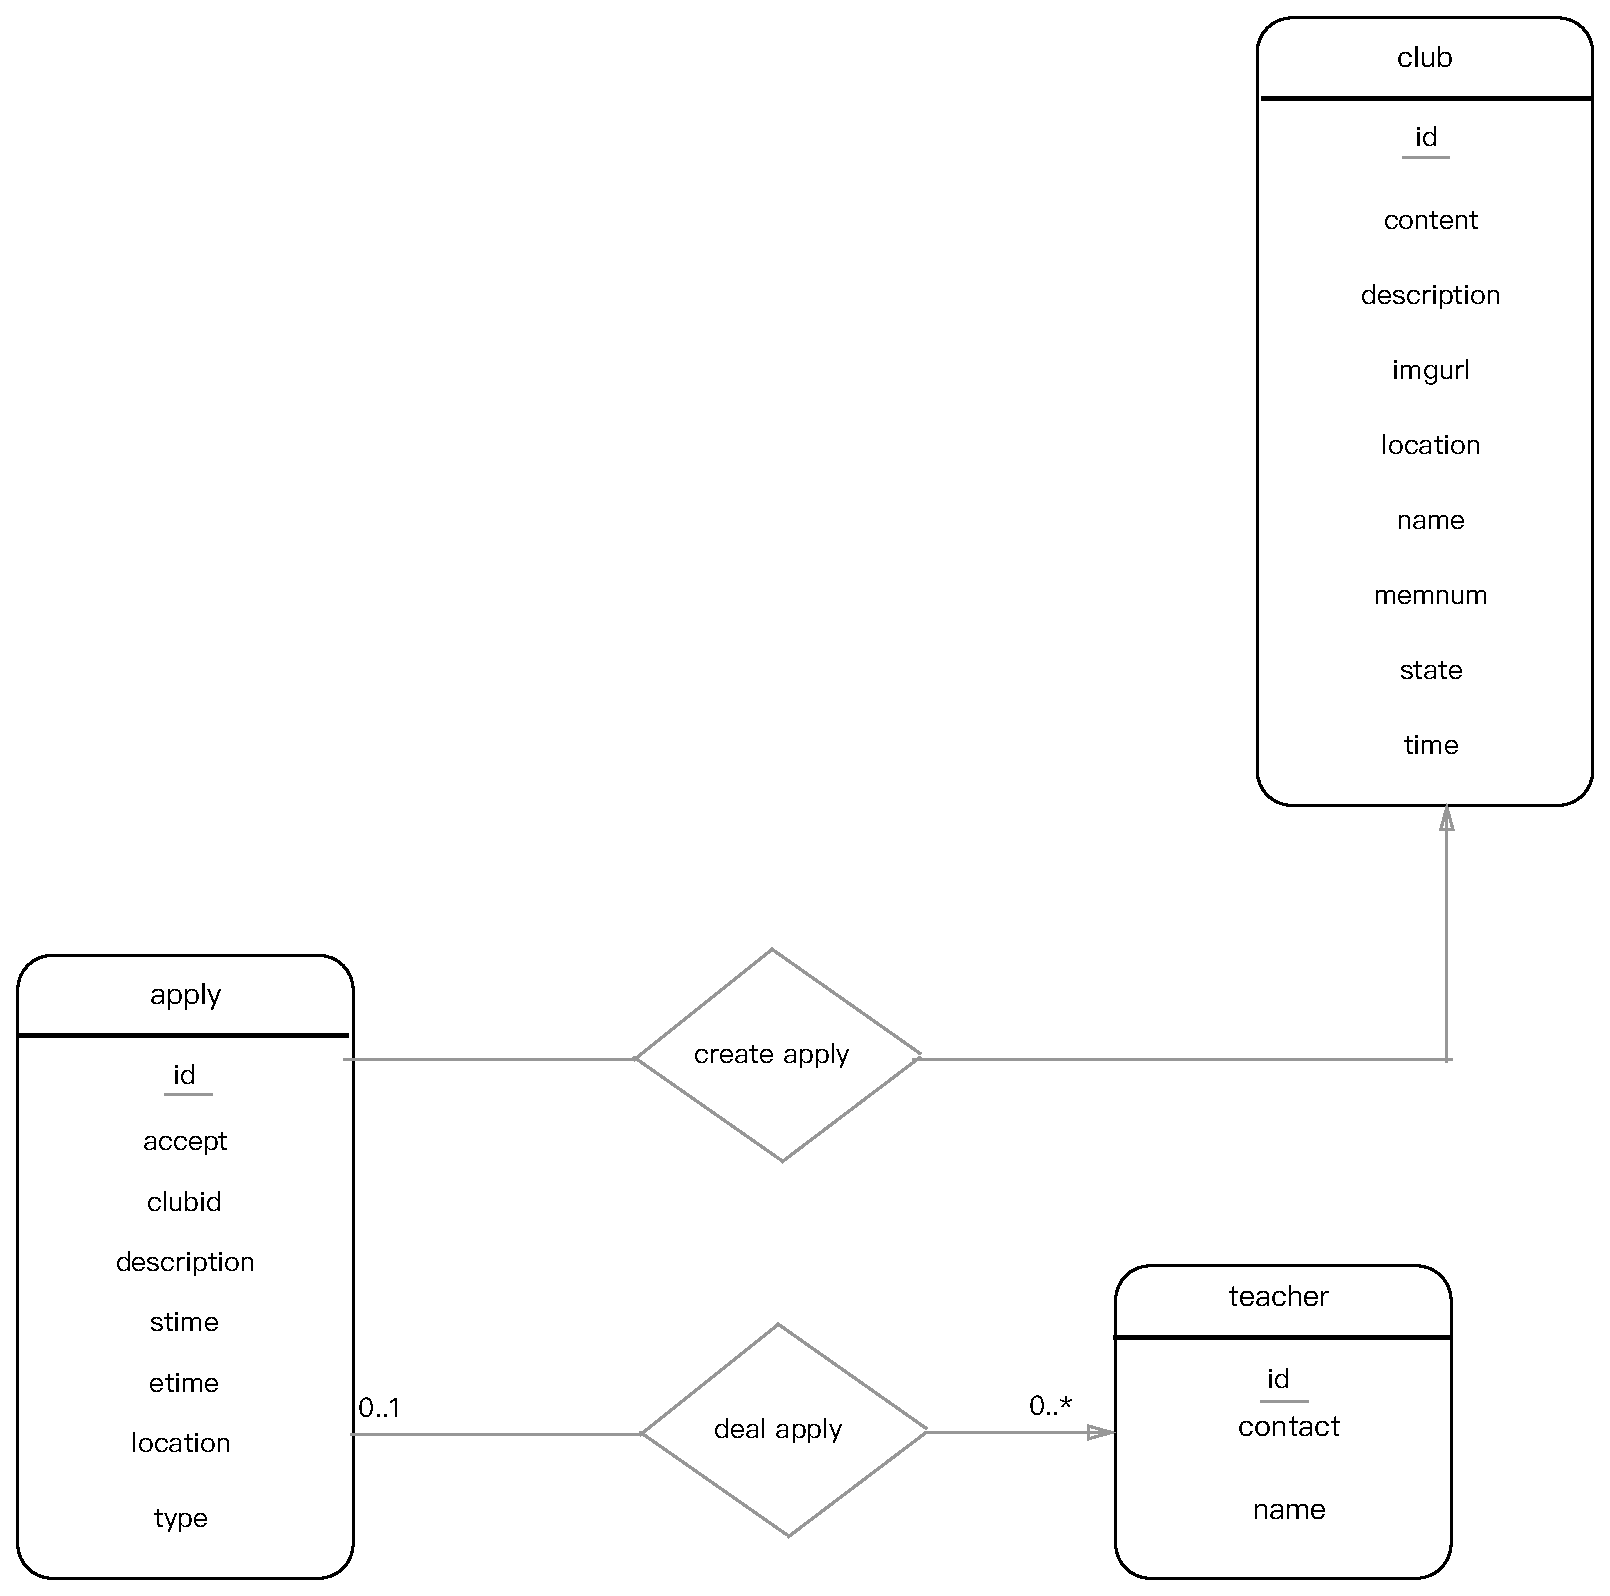
\includegraphics[width = 0.8\textwidth]{apply-*-er.eps}
\end{figure}

\paragraph{实体(Entity)}
本系统中的实体类主要为Student、Teacher、Club、Activity、Apply、Comment、ClubFile:
\begin{figure}[H]
\centering
\includegraphics[width = 1.0\textwidth]{xianhuo-class.png}
\end{figure}

\subparagraph{Student}
Student为本系统中普通用户、社团负责人和老师的实体,Teacher继承自Student,具体属性和方法如下图:
\newline
\begin{figure}[H]
\centering
\includegraphics[width = 0.5\textwidth]{student-class.png}
\end{figure}
\begin{table}[H]
\centering
\caption{Student类}
\begin{tabular}{|c|c|c|c|c|c|}
\hline
\multicolumn{6}{|c|}{Student}\\
\hline
类别& 名称& 类型 & 参数 & 返回类型& 备注\\
\hline
\multirow{9}*{属性}
&id & String & 无 & 无 & 学生的学号\\
&name & String & 无 & 无 & 学生的姓名\\
&grade& String & 无 & 无 & 学生的年级\\
&major& String & 无 & 无 & 学生的专业\\
&password& String & 无 & 无 & 学生的密码\\
&headimg& String & 无 & 无 & 学生的头像\\
&contact& String & 无 & 无 & 学生的号码\\
&clubs& List<Club> & 无 & 无 & 学生的参加的社团\\
&activities& List<Activity> & 无 & 无 & 学生参加的活动\\
\hline
\multirow{18}*{方法}
&setId & 无 & String & void & 设置学生的学号\\
&getId & 无 & 无 & String & 得到学生的学号\\
&setName & 无 & String & void & 设置学生的名字\\
&getName & 无 & 无 & String & 得到学生的姓名\\
&setGrade & 无 & String & void & 设置学生的年级\\
&getGrade & 无 & 无 & String & 得到学生的年级\\
&setMajor & 无 & String & void & 设置学生的专业\\
&getMajor & 无 & 无 & String & 得到学生的专业\\
&setPassword & 无 & String & void & 设置学生的密码\\
&getPassword & 无 & 无 & String & 得到学生的密码\\
&setContact & 无 & String & void & 设置学生的联系方式\\
&getContact & 无 & 无 & String & 得到学生的联系方式\\
&setClubs & 无 & List<Club> & void & 设置学生参加的社团\\
&getClubs & 无 & 无 & String & 得到学生的参加的社团\\
&setHeadImg & 无 & String & void & 设置学生的头像\\
&getHeadImg & 无 & 无 & String & 得到学生的头像\\
&setActivities & 无 & List<Activity> & 无 & 设置学生参加的活动\\
&getActivities & 无 & 无 & List<Activity> & 得到学生参加的活动\\
\hline
\end{tabular}
\end{table}

\subparagraph{Teacher}
Teacher是本系统中管理社团创建和场地申请的老师的实体类,它继承自Student,拥有新的属性applies,具体信息如下图:
\newline
\begin{figure}[H]
\centering
\includegraphics[width = 0.5\textwidth]{teacher-class.png}
\end{figure}
\begin{table}[H]
\centering
\caption{Teacher类}
\begin{tabular}{|c|c|c|c|c|c|}
\hline
\multicolumn{6}{|c|}{Teacher}\\
\hline
类别& 名称& 类型 & 参数 & 返回类型& 备注\\
\hline
\multirow{1}*{属性}
&applies& List<Apply> & 无 & 无 & 老师收到的请求列表\\
\hline
\multirow{2}*{方法}
&setApplies & 无 & List<Apply> & 无 & 设置老师收到的请求\\
&getApplies & 无 & 无 & List<Apply> & 得到老师收到的请求\\
\hline
\end{tabular}
\end{table}

\subparagraph{Activity}
Activity为本系统中社团活动的实体类,具体属性和方法如下图:
\newline
\begin{figure}[H]
\centering
\includegraphics[width = 0.5\textwidth]{activity-class.png}
\end{figure}
\begin{table}[H]
\centering
\caption{Activity类}
\begin{tabular}{|c|c|c|c|c|c|}
\hline
\multicolumn{6}{|c|}{Activity}\\
\hline
类别& 名称& 类型 & 参数 & 返回类型& 备注\\
\hline
\multirow{12}*{属性}
&id & Long & 无 & 无 & 活动的id\\
&name & String & 无 & 无 & 活动的名称\\
&location& String & 无 & 无 & 活动地点\\
&time& Date & 无 & 无 & 活动时间\\
&contact& String & 无 & 无 & 联系方式\\
&number& Integer & 无 & 无 & 参加人数\\
&imgUrl& String & 无 & 无 & 宣传的图片\\
&description& String & 无 & 无 & 活动的描述\\
&state& boolean & 无 & 无 & 活动状态\\
&studentList& List<Student> & 无 & 无 & 参加的学生列表\\
&commentList& List<Comment> & 无 & 无 & 评论列表\\
\hline
\multirow{22}*{方法}
&setId & 无 & Long & void & 设置活动的id\\
&getId & 无 & 无 & Long & 得到活动的id\\
&setName & 无 & String & void & 设置活动的名称\\
&getName & 无 & 无 & String & 得到活动的名称\\
&setLocation & 无 & String & void & 设置活动的地点\\
&getLocation & 无 & 无 & String & 得到活动的地点\\
&setTime & 无 & Date & void & 设置活动的时间\\
&getTime & 无 & 无 & Date & 得到活动的时间\\
&setContact & 无 & String & void & 设置活动的联系方式\\
&getContact & 无 & 无 & String & 得到活动的联系方式\\
&setNumber & 无 & Integer & void & 设置参加活动的人数\\
&getNumber & 无 & 无 & Integer & 得到参加活动的人数\\
&setImgUrl & 无 & String & void & 设置活动的宣传图片\\
&getImgUrl & 无 & 无 & String & 得到活动的宣传图片\\
&setDescription & 无 & String & void & 设置活动的描述\\
&getDescription & 无 & 无 & String & 得到活动的描述\\
&setState & 无 & boolean & void & 设置活动的状态\\
&getState & 无 & 无 & boolean & 得到活动的状态\\
&setStudentList & 无 & List<Student> & void & 设置活动的参加学生\\
&getStudentList & 无 & 无 & List<Student> & 得到活动的参加学生\\
&setCommentList & 无 & List<Comment> & void & 设置活动的评论\\
&getCommentList & 无 & 无 & List<Comment> & 得到活动的评论\\
\hline
\end{tabular}
\end{table}

\subparagraph{Apply}
Apply为本系统中由社团负责人发起的场地申请或海报申请的实体类,具体信息如下:
\newline
\begin{figure}[H]
\centering
\includegraphics[width = 0.5\textwidth]{apply-class.png}
\end{figure}
\begin{table}[H]
\centering
\caption{Apply类}
\begin{tabular}{|c|c|c|c|c|c|}
\hline
\multicolumn{6}{|c|}{Apply}\\
\hline
类别& 名称& 类型 & 参数 & 返回类型& 备注\\
\hline
\multirow{8}*{属性}
&id & Long & 无 & 无 & 申请的id\\
&clubId & Long & 无 & 无 & 发起申请的社团的id\\
&type& Integer & 无 & 无 & 申请的类型\\
&startDate& Date & 无 & 无 & 申请的开始时间节点\\
&endDate& Date & 无 & 无 & 申请的结束时间节点\\
&location& String & 无 & 无 & 申请的地点\\
&description& String & 无 & 无 & 申请的理由\\
&accept& Integer & 无 & 无 & 申请的状态\\
\hline
\multirow{16}*{方法}
&setId & 无 & Long & void & 设置申请的id\\
&getId & 无 & 无 & Long & 得到申请的id\\
&setClubId & 无 & Long & void & 设置申请的社团的id\\
&getClubId & 无 & 无 & Long & 得到申请的社团的id\\
&setType & 无 & Integer & void & 设置申请的类型\\
&getType & 无 & 无 & Integer & 得到申请的类型\\
&setStartTime & 无 & Date & void & 设置申请的开始的时间节点\\
&getEndTime & 无 & 无 & Date & 得到申请的开始的时间节点\\
&setEndTime & 无 & Date & void & 设置申请的结束的时间节点\\
&getEndTime & 无 & 无 & Date & 得到申请的结束的时间节点\\
&setLocation & 无 & String & void & 设置申请的地点\\
&getLocation & 无 & 无 & String & 得到申请的地点\\
&setDescription & 无 & String & void & 设置申请的理由\\
&getDescription & 无 & 无 & String & 得到申请理由\\
&setAccept & 无 & Integer & void & 设置申请的状态\\
&getAccept & 无 & 无 & Integer & 得到申请的状态\\
\hline
\end{tabular}
\end{table}

\subparagraph{Club}
Club为本系统中的核心类,几乎所有操作都会跟这个实体类有一定的关系,其属性和方法也比较多,具体信息如下:
\newline
\begin{figure}[H]
\centering
\includegraphics[width = 0.5\textwidth]{club-class.png}
\end{figure}
\begin{table}[H]
\centering
\caption{Club类}
\begin{tabular}{|c|c|c|c|c|c|}
\hline
\multicolumn{6}{|c|}{Club}\\
\hline
类别& 名称& 类型 & 参数 & 返回类型& 备注\\
\hline
\multirow{13}*{属性}
&id & Long & 无 & 无 & 社团的id\\
&name & String & 无 & 无 & 社团的名称\\
&state& Integer & 无 & 无 & 社团的审核状态\\
&teacher& String & 无 & 无 & 社团的指导老师\\
&chairmanId& String & 无 & 无 & 社团主席的id\\
&menberNumber& Integer & 无 & 无 & 社员人数\\
&imgUrl& String & 无 & 无 & 社团的展示封面\\
&description& String & 无 & 无 & 社团的描述\\
&content& String & 无 & 无 & 社团申请标语\\
&students& List<Student> & 无 & 无 & 社员列表\\
&activities& List<Activity> & 无 & 无 & 活动列表\\
&comments& List<Comment> & 无 & 无 & 评论列表\\
&clubFiles& List<clubFile> & 无 & 无 & 资源文件列表\\
\hline
\multirow{26}*{方法}
&setId & 无 & Long & void & 设置社团的id\\
&getId & 无 & 无 & Long & 得到社团的id\\
&setName & 无 & String & void & 设置社团的名称\\
&getName & 无 & 无 & String & 得到社团的名称\\
&setState & 无 & Integer & void & 设置社团的审核状态\\
&getState & 无 & 无 & Integer & 得到社团的审核状态\\
&setTeacher & 无 & String & void & 设置社团的指导老师\\
&getTeacher & 无 & 无 & String & 得到社团的指导老师\\
&setChairManId & 无 & String & void & 设置社团的主席id\\
&getChairManId & 无 & 无 & String & 得到社团的主席id\\
&setContent & 无 & String & void & 设置社团的申请标语\\
&getContent & 无 & 无 & String & 得到社团的申请标语\\
&setMemberNumber & 无 & Integer & void & 设置参加社员的人数\\
&getMenberNumber & 无 & 无 & Integer & 得到参加社员的人数\\
&setImgUrl & 无 & String & void & 设置社团的封面图片\\
&getImgUrl & 无 & 无 & String & 得到社团的封面图片\\
&setDescription & 无 & String & void & 设置社团的描述\\
&getDescription & 无 & 无 & String & 得到社团的描述\\
&setStudents & 无 & List<Student> & void & 设置社员\\
&getStudents & 无 & 无 & List<Student> & 得到社员\\
&setComments & 无 & List<Comment> & void & 设置社团的评论\\
&getComments & 无 & 无 & List<Comment> & 得到社团的评论\\
&setActivities & 无 & List<Activity> & 无 & 设置社团活动\\
&getActivities & 无 & 无 & List<Activity> & 得到社团的活动\\
&setClubFiles & 无 & List<ClubFile> & 无 & 设置社团资源文件\\
&getClubFiles & 无 & 无 & List<ClubFile> & 得到社团资源文件\\
\hline
\end{tabular}
\end{table}

\subparagraph{Comment}
Comment为本系统中评论的实体类,由Student创建,跟Club和Activity相关联,具体信息如下:
\newline
\begin{figure}[H]
\centering
\includegraphics[width = 0.5\textwidth]{comment-class.png}
\end{figure}
\begin{table}[H]
\centering
\caption{Comment类}
\begin{tabular}{|c|c|c|c|c|c|}
\hline
\multicolumn{6}{|c|}{Comment}\\
\hline
类别& 名称& 类型 & 参数 & 返回类型& 备注\\
\hline
\multirow{8}*{属性}
&id & Long & 无 & 无 & 评论的id\\
&studentId & String & 无 & 无 & 发起评论学生的id\\
&targetId& Long & 无 & 无 & 评论目标的id\\
&targetType& Integer & 无 & 无 & 评论目标的类别\\
&content& String & 无 & 无 & 评论的内容\\
&activity& Activity & 无 & 无 & 评论的活动\\
&club& Club & 无 & 无 & 评论的社团\\
&date& Date & 无 & 无 & 评论的时间\\
\hline
\multirow{16}*{方法}
&setId & 无 & Long & void & 设置评论的id\\
&getId & 无 & 无 & Long & 得到评论的id\\
&setStudentId & 无 & String & void & 设置评论学生的id\\
&getStudentId & 无 & 无 & String & 得到评论学生的id\\
&setTargetId & 无 & Long & void & 设置评论目标的id\\
&getTargetId & 无 & 无 & Long & 得到评论目标的id\\
&setTargetType & 无 & Integer & void & 设置评论目标的类别\\
&getTargetType & 无 & 无 & Integet & 得到评论目标的类别\\
&setContent & 无 & String & void & 设置评论内容\\
&getContent & 无 & 无 & String & 得到评论内容\\
&setActivity & 无 & Activity & 无 & 设置评论的活动\\
&getActivity & 无 & 无 & Activity & 得到评论的活动\\
&setClub & 无 & Club & 无 & 设置评论的社团\\
&getClub & 无 & 无 & Club & 得到评论的社团\\
\hline
\end{tabular}
\end{table}

\subparagraph{ClubFile}
ClubFile为本系统中社团资源文件的实体类,由Club创建,由七牛云托管,具体信息如下:
\newline
\begin{figure}[H]
\centering
\includegraphics[width = 0.5\textwidth]{clubfile-class.png}
\end{figure}
\begin{table}[H]
\centering
\caption{ClubFile类}
\begin{tabular}{|c|c|c|c|c|c|}
\hline
\multicolumn{6}{|c|}{ClubFile}\\
\hline
类别& 名称& 类型 & 参数 & 返回类型& 备注\\
\hline
\multirow{4}*{属性}
&id & Long & 无 & 无 & 资源文件的id\\
&name & String & 无 & 无 & 资源文件的名称\\
&url& String & 无 & 无 & 资源文件的下载地址\\
&clubId& Long & 无 & 无 & 对应社团的id\\
\hline
\multirow{8}*{方法}
&setId & 无 & Long & void & 设置资源文件的id\\
&getId & 无 & 无 & Long & 得到资源文件的id\\
&setName & 无 & String & void & 设置资源文件的名称\\
&getName & 无 & 无 & String & 得到资源文件的名称\\
&setUrl & 无 & String & void & 设置资源文件的下载地址\\
&getUrl & 无 & 无 & String & 得到资源文件的下载地址\\
&setClubId & 无 & Long & void & 设置对应社团的id\\
&getClubId & 无 & 无 & Long & 得到对应社团的id\\
\hline
\end{tabular}
\end{table}

\paragraph{仓库类和服务类(repository \& Service)}
仓库类和服务类是本项目中不可或缺的一部分,它们管理着实例,为上层的controller提供数据支持,其类图如下:
\newline
\begin{figure}[H]
\centering
\includegraphics[width = 1.1\textwidth]{repository-service.png}
\end{figure}

\subparagraph{StudentRepository \& StudentService}
StudentRepository和StudentService在本系统中担任管理学生业务的重任,对实体类Student进行一层封装,使其增删改查变的非常容易,以下为其具体细节,因为StudentService为StudentRepository的实现,所以具体介绍StudentService:
\newline
\begin{figure}[H]
\centering
\includegraphics[width = 0.4\textwidth]{student-rs.png}
\end{figure}
\begin{center}
\emph{save(Student student):void}\\
修改数据库中学生信息\\ 
\emph{findById(String Id):List<Student>}\\
根据学生id在数据库中查找学生\\
\emph{addStudent(String Id, String Name, String Grade, String Major, String Contact, String Password):void}\\
根据学生完整信息生成学生存入数据库\\
\emph{getStudentActivity(String Id):List<Activity>}\\
根据学生学号查到某学生并获得他所有的活动\\
\emph{login(String Id, String Password):Integer}\\
对某学生执行登录操作
\end{center}

\subparagraph{ClubRepository \& ClubService}
ClubRepository和ClubService在本系统中担任管理社团业务的重任,对实体类Club进行一层封装,使其增删改查变得非常容易,以下为具体细节,因为ClubService为ClubRepository的实现,所以具体介绍ClubService:
\newline
\begin{figure}[H]
\centering
\includegraphics[width = 0.4\textwidth]{club-rs.png}
\end{figure}
\begin{center}
\emph{save(Club club):void}\\
修改数据库中社团的信息\\
\emph{findById(Long Id):List<Club>}\\
根据社团的id查找到社团\\
\emph{findAll():List<Club>}\\
将所有的社团信息返回\\
\emph{studentQuitClub(Long id, String id):boolean}\\
将一个学生退出社团\\
\emph{studentApplyClub(Long id, String id):boolean}\\
学生申请加入社团\\
\emph{addCommentToClub(Comment comment, Long id):void}\\
对俱乐部进行评论\\
\end{center}

\subparagraph{ActivityRepository \& ActivityService}
ActivityRepository和ActivityService在本系统中担任管理活动业务的重任,对实体类Activity进行一层封装,使其增删改查变得非常容易,以下为具体细节,因为ActivityService为ActivityRepository的实现,所以具体介绍ActivityService:
\newline
\begin{figure}[H]
\centering
\includegraphics[width = 0.4\textwidth]{activity-rs.png}
\end{figure}
\begin{center}
\emph{save(Activity activity):void}\\
修改数据库中活动的信息\\
\emph{findById(Long Id):List<Activity>}\\
根据活动的id查找到活动\\
\emph{findAll():List<Activity>}\\
将所有的活动信息返回\\
\emph{addStudentToActivity(String id, Long id):void}\\
将一个学生加入一个活动中\\
\emph{deleteStudentFromActivity(String id, Long id):void}\\
将一个学生从一个活动中删除\\
\emph{addCommentToActivity(Comment comment, Long id):void}\\
对活动进行评论
\end{center}

\subparagraph{ApplyRepository \& ApplyService}
ApplyRepository和ApplyService在本系统中担任管理请求业务的重任,对实体类Apply进行一层封装,使其增删改查变得非常容易,以下为具体细节,因为ApplyService为ApplyRepository的实现,所以具体介绍ApplyService:
\newline
\begin{figure}[H]
\centering
\includegraphics[width = 0.4\textwidth]{apply-rs.png}
\end{figure}
\begin{center}
\emph{save(Apply apply):void}\\
修改数据库中请求的信息\\
\emph{findById(Long Id):List<Apply>}\\
根据请求的Id查找到请求\\
\emph{findAll():List<Apply>}\\
返回全部请求
\end{center}

\subparagraph{CommentRepository \& CommentService}
CommentRepository和CommentService在本系统中担任管理评论业务的重任,对实体类Comment进行一层封装,使其增删改查变得非常容易,以下为具体细节,因为CommentService为CommentRepository的实现,所以具体介绍CommentService:
\newline
\begin{figure}[H]
\centering
\includegraphics[width = 0.4\textwidth]{comment-rs.png}
\end{figure}
\begin{center}
\emph{save(Comment comment):void}\\
修改数据库中评论的信息\\
\emph{findById(Long Id):List<Comment>}\\
根据请求的Id查找到评论\\
\emph{findAllCommentOfClub(Long Id):List<Comment>}\\
返回某个社团的所有评论\\
\emph{findAllCommentOfActivity(Long Id):List<Comment>}\\
返回某个活动的所有评论
\end{center}

\subparagraph{FileRepository \& FileService}
ClubFileRepository和ClubFileService在本系统中担任管理社团资源文件业务的重任,对实体类ClubFile进行一层封装,使其增删改查变得非常容易,以下为具体细节,因为ClubFileService为ClubFileRepository的实现,所以具体介绍ClubFileService:
\newline
\begin{figure}[H]
\centering
\includegraphics[width = 0.4\textwidth]{clubfile-rs.png}
\end{figure}
\begin{center}
\emph{save(ClubFile clubFile):void}\\
修改数据库中俱乐部资源文件的信息
\end{center}

\subparagraph{EncryptionService}
EncryptionService为学生的登录提供MD5加密服务,在每次登录的时候这个服务类都会把明文密码转化为用MD5加密的密文,以下为具体细节:
\newline
\begin{figure}[H]
\centering
\includegraphics[width = 0.4\textwidth]{Encryption-rs.png}
\end{figure}
\begin{center}
\emph{encipherPassword(String Password):String}\\
将给定的明文密码转化为MD5密文\\
\emph{checkByPython(String Id, String Password):boolean}\\
使用python脚本访问4m3本研一体化网站验证账号\\
\emph{comparePW(String Id, String Password):boolean}\\
比对用户的账号和密码是不是和数据库中的吻合\\
\emph{encipher(String Password):String}\\
对密文进行撒盐\\
\emph{checkIdentity(String Id, String Password):boolean}\\
验明身份并写session
\end{center}

\subsubsection{行为建模}
张

\section{UI 需求}
本项目的web端将使用主流的简约风格,而“同心云”端将使用契合iphone手机界面的ios风。
\subsection{web端}
本项目面向的对象是同济大学全体师生,是一个年轻的群体,需要一个富有青春活力的界面风格和设计。本系统将把界面分为首页、登录页、活动页、社团页、个人管理中心和老师审核中心6个大的版块,以下为具体的页面跳转关系:
\newline
\begin{figure}[H]
\centering
\includegraphics[width = 1.0\textwidth]{web.eps}
\end{figure}

\subsubsection{首页}
\begin{figure}[H]
\centering
\includegraphics[width = .9\textwidth]{web-index.png}
\end{figure}
\paragraph{页面简介}
首页将介绍平台的几大板块并提供跳转链接,让用户一目了然地了解平台的作用。

\paragraph{组成元素及说明}
\subparagraph*{导航栏}
导航栏位于页面顶端,左侧提供首页、活动首页、社团首页的跳转链接,右侧提供搜索栏和登录链接。如果用户处于登录的状态,将登录按钮置换成用户管理中心的跳转链接。
\subparagraph*{巨幕}
首页的巨幕显示平台的名称和宣传标语。
\subparagraph*{板块简介}
板块简介分为两个部分,第一个部分是社团管理功能的简介,将提供社团首页的跳转链接;第二部分是活动管理功能的简介,将提供活动首页的跳转链接。
\subparagraph*{页脚}
页脚将提供平台的联系方式和开发者相关信息。

\subsubsection{登录}
\begin{figure}[H]
\centering
\includegraphics[width = .9\textwidth]{web-login.png}
\end{figure}
\paragraph{页面简介}
登录页将提供一个用于登录的表单,用户通过输入自己在同济大学的学号和同意认证账号即可登录并跳转到首页。管理员账号将直接跳转到管理页面进行相关的管理。

\paragraph{组成元素及说明}
\subparagraph*{导航栏}
导航栏位于页面顶端,左侧提供首页、活动首页、社团首页的跳转链接,右侧提供搜索栏和登录链接。如果用户处于登录的状态,将登录按钮置换成用户管理中心的跳转链接。
\subparagraph*{巨幕}
巨幕说明当前页面是登录页面
\subparagraph*{登录表单}
登录表单将提供学号输入框和密码输入框,输入学号和密码之后点击登录即可登录并跳转到首页。如果密码错误将出现密码错误的提示,页面不发生跳转。
\subparagraph*{页脚}
页脚将提供平台的联系方式和开发者相关信息。

\subsubsection{活动}
\begin{figure}[H]
\centering
\includegraphics[width = .9\textwidth]{web-activity-home.png}
\end{figure}
\paragraph{页面简介}
活动首页将列出当前处于活跃期的活动列表,用户在登录状态下还将可以看到自己当前参加的活动,如果是社团负责人,将在登录状态下看到自己创建的社团活动,该页将为这些活动提供快速的跳转链接。

\paragraph{组成元素及说明}
\subparagraph*{导航栏}
导航栏位于页面顶端,左侧提供首页、活动首页、社团首页的跳转链接,右侧提供搜索栏和登录链接。如果用户处于登录的状态,将登录按钮置换成用户管理中心的跳转链接。
\subparagraph*{巨幕}
巨幕将说明当前页面是活动首页。
\subparagraph*{公共活动列表}
公共活动列表用卡片样式输出活动,活动卡片将包含以下信息:活动名称、活动时间、活动地点、活动简要描述和跳转链接。
\subparagraph*{个人活动列表}
在登录状态下,用户将可以在页面的右侧看到一个标签页,标签页第一页为自己当前参加的活动列表,第二页为自己创建的活动,提供相应的超链接。
\subparagraph*{页脚}
页脚将提供平台的联系方式和开发者相关信息。

\subsubsection{活动细节}
\begin{figure}[H]
\centering
\includegraphics[width = .9\textwidth]{web-activity-detail.png}
\end{figure}
\paragraph{页面简介}
活动细节页面将向用户展示活动的具体信息,包括活动名称、地点、时间、主办方等。在登录状态下,用户可以注册参加这项活动,并可以参与活动的评论,即使处于未登录状态,也可以看到相关评论。

\paragraph{组成元素及说明}
\subparagraph*{导航栏}
导航栏位于页面顶端,左侧提供首页、活动首页、社团首页的跳转链接,右侧提供搜索栏和登录链接。如果用户处于登录的状态,将登录按钮置换成用户管理中心的跳转链接。
\subparagraph*{巨幕}
巨幕将说明当前页面是活动细节页面,同时,巨幕的背景会被换成活动的宣传图片。
\subparagraph*{左侧宣传画}
页面左侧将展现该活动的宣传画。
\subparagraph*{参与活动注册按钮}
用户在登录状态下,将看到有一个按钮位于宣传画的下方,如果未注册该活动,按钮为绿色并显示“参加活动”,若用户已经参加,则为红色,显示“退出活动”
\subparagraph*{右侧活动详情列表}
右侧的活动详情列表将显示该活动的一些具体信息。
\subparagraph*{右侧评论区}
右侧的评论区将列出对当前活动的评论。
\subparagraph*{页脚}
页脚将提供平台的联系方式和开发者相关信息。

\subsubsection{社团}
\begin{figure}[H]
\centering
\includegraphics[width = .9\textwidth]{web-club-home.png}
\end{figure}
\paragraph{页面简介}
社团首页将列出当前所有的社团,用户在登录状态下还将可以看到自己当前参加的社团,如果是社团负责人,将在登录状态下看到自己创建的社团,该页将为这些社团提供快速的跳转链接。

\paragraph{组成元素及说明}
\subparagraph*{导航栏}
导航栏位于页面顶端,左侧提供首页、活动首页、社团首页的跳转链接,右侧提供搜索栏和登录链接。如果用户处于登录的状态,将登录按钮置换成用户管理中心的跳转链接。
\subparagraph*{巨幕}
巨幕将说明当前页面是社团首页页面。
\subparagraph*{社团列表}
社团列表将以卡片样式输出所有的社团,并显示社团宣传画、社团名称、指导老师、简要描述和社员总人数等信息。
\subparagraph*{个人社团列表}
在登录状态下,用户将可以在页面的右侧看到一个标签页,标签页第一页为自己当前参加的社团列表,第二页为自己创建的社团列表,提供相应的超链接。
\subparagraph*{页脚}
页脚将提供平台的联系方式和开发者相关信息。

\subsubsection{社团细节}
\begin{figure}[H]
\centering
\includegraphics[width = .9\textwidth]{web-club-detail.png}
\end{figure}
\paragraph{页面简介}
社团细节页面将向用户展示社团的具体信息,包括社团名称、指导老师、简介等信息。在登录状态下,用户可以注册参加这项社团,并可以参与社团的评论,同时还可以看到并下载社团的资源文件,但即使处于未登录状态,也可以看到相关评论,只是看不到资源文件。

\paragraph{组成元素及说明}
\subparagraph*{导航栏}
导航栏位于页面顶端,左侧提供首页、活动首页、社团首页的跳转链接,右侧提供搜索栏和登录链接。如果用户处于登录的状态,将登录按钮置换成用户管理中心的跳转链接。
\subparagraph*{巨幕}
巨幕将说明当前页面是社团细节页面,同时,巨幕的背景会被换成社团的宣传图片。
\subparagraph*{左侧宣传画}
页面左侧将展现该社团的宣传画。
\subparagraph*{参与社团注册按钮}
用户在登录状态下,将看到有一个按钮位于宣传画的下方,如果未注册该社团,按钮为绿色并显示“参加社团”,若用户已经参加,则为红色,显示“退出社团”。
\subparagraph*{资源文件按钮 \& 资源文件列表}
用户在登录并参与了该社团的情况下,将可以看到宣传画下方有一个资源文件按钮,点击该按钮将显示资源文件列表,若未注册该社团,该按钮将被禁用。
\subparagraph*{右侧社团详情列表}
右侧的活动详情列表将显示该社团的一些具体信息。
\subparagraph*{右侧评论区}
右侧的评论区将列出对当前社团的评论。
\subparagraph*{页脚}
页脚将提供平台的联系方式和开发者相关信息。

\subsubsection{社团管理}
\begin{figure}[H]
\centering
\includegraphics[width = .9\textwidth]{web-club-admin.png}
\end{figure}
\paragraph{页面简介}
社团管理页面将由资源区管理、活动管理、学生、申请、个性化推荐五个版块组成,同时提供编辑社团信息的功能。

\paragraph{组成元素及说明}
\subparagraph*{导航栏}
导航栏位于页面顶端,左侧提供首页、活动首页、社团首页的跳转链接,右侧提供搜索栏和登录链接。如果用户处于登录的状态,将登录按钮置换成用户管理中心的跳转链接。
\subparagraph*{巨幕}
巨幕将说明当前页面是社团管理页面,同时,巨幕的背景会被换成社团的宣传图片。
\subparagraph*{左侧宣传画}
页面左侧将展现该社团的宣传画。点击该画将显示更换头像的按钮,选择更换头像就可以上传图片更换社团的宣传画。宣传画下方有编辑社团信息的按钮,点击并填写相关内容就可以更改社团的相关信息。
\subparagraph*{资源区管理}
资源区管理将提供上传资源文件的按钮,点击即可上传文件,同时将会有资源文件列表供查看并可以执行删除资源文件的操作。
\subparagraph*{活动管理}
活动管理区将提供创建活动的按钮,填完信息即可创建相关活动,同时下方将提供当前社团所有活动的列表,并提供相应链接和通知全体社员该活动信息的功能。
\subparagraph*{学生管理}
学生管理区可以看到当前所有参加这个社团的学生,并提供了一个群发短信的按钮,点击并输入按钮就可以发送信息。
\subparagraph*{申请管理}
申请管理区可以向老师提交申请,申请场地或者申请张贴海报,并提供一个申请列表查看当前的所有申请的状态,通过为绿色,拒绝为红色,等待中为黄色。
\subparagraph*{个性化推荐}
个性化推荐区将推送由系统提供的相关活动的建议。
\subparagraph*{页脚}
页脚将提供平台的联系方式和开发者相关信息。

\subsubsection{管理中心}
\begin{figure}[H]
\centering
\includegraphics[width = .9\textwidth]{web-center.png}
\end{figure}
\paragraph{页面简介}
个人管理中心页面将显示用户的个人信息和用户当前参加的社团列表、当前参加的活动列表和当前创建的社团列表。并提供编辑个人信息的功能。

\paragraph{组成元素及说明}
\subparagraph*{导航栏}
导航栏位于页面顶端,左侧提供首页、活动首页、社团首页的跳转链接,右侧提供搜索栏和登录链接。如果用户处于登录的状态,将登录按钮置换成用户管理中心的跳转链接。
\subparagraph*{巨幕}
巨幕将说明当前页面是个人信息管理页面,同时,巨幕的背景会被换成个人的头像。
\subparagraph*{左侧个人信息}
页面左侧将展现该用户的基本个人信息。点击用户头像显示更换头像的按钮,选择更换头像就可以上传图片更换用户头像。头像下方有编辑个人信息的按钮,点击并填写相关内容就可以更改个人的相关信息。
\subparagraph*{参加的社团列表}
参加的社团列表将对用户参加的社团进行打表输出,并提供详情页面跳转的功能。
\subparagraph*{参加的活动列表}
参加的活动列表将对用户参加的活动进行打表输出,并提供详情页面跳转的功能。
\subparagraph*{创建的社团列表}
参加的社团列表将对用户参加的社团进行打表输出,并提供详情页面和管理页面跳转的功能。
\subparagraph*{页脚}
页脚将提供平台的联系方式和开发者相关信息。

\subsubsection{审核中心}
\begin{figure}[H]
\centering
\includegraphics[width = .9\textwidth]{web-admin.png}
\end{figure}
\paragraph{页面简介}
总管理页面将显示老师的信息和当前社团的申请请求队列和场地的申请请求队列,老师可以在这里对请求进行操作,同意或者拒绝。

\paragraph{组成元素及说明}
\subparagraph*{导航栏}
导航栏位于页面顶端,左侧提供首页、活动首页、社团首页的跳转链接,右侧提供搜索栏和登录链接。如果用户处于登录的状态,将登录按钮置换成用户管理中心的跳转链接。
\subparagraph*{巨幕}
巨幕将说明当前页面是总管理页面,同时,巨幕的背景会被换成老师的个人的头像。
\subparagraph*{左侧个人信息}
页面左侧将展现该老师的基本个人信息。点击用户头像显示更换头像的按钮,选择更换头像就可以上传图片更换用户头像。头像下方有编辑个人信息的按钮,点击并填写相关内容就可以更改个人的相关信息。
\subparagraph*{社团创建请求列表}
社团创建请求列表将列出所有申请创建的社团的请求,老师可以查看其信息然后决定是否同意。
\subparagraph*{场地申请请求列表}
场地申请请求列表将列出所有场地申请的请求,老师可以查看其信息然后决定是否同意。
\subparagraph*{页脚}
页脚将提供平台的联系方式和开发者相关信息。

\subsection{“同心云”端}
”同心云“端将使用ios风格的界面,简单展示活动和社团详情,以下为具体的页面跳转关系:
\newline
\begin{figure}[H]
\centering
\includegraphics[width = 1.0\textwidth]{tongxinyun.eps}
\end{figure}

\subsubsection{首页}
\begin{figure}[H]
\centering
\includegraphics[width = .5\textwidth]{tong-index.png}
\end{figure}
\paragraph{页面简介}
首页将显示该用户的个人基础信息并提供该用户参加的活动和社团的列表,并可以查看到自己的评论信息。

\paragraph{组成元素及说明}
\subparagraph*{个人信息}
由于移动端屏幕较小,该页个人信息只输出头像、学号和姓名,并不支持修改,个人信息置于该页顶部。
\subparagraph*{我的社团列表}
我的社团列表将跳转到另一页显示该用户参加的社团。
\subparagraph*{我的活动列表}
我的活动列表将跳转到另一页显示该用户参加的活动。
\subparagraph*{我的评论列表}
我的评论列表将跳转到另一页显示该用户发起的评论。
\subparagraph*{底栏}
底栏将提供首页、活动、社团、信息中心的跳转链接。

\subsubsection{活动}
\begin{figure}[H]
\centering
\includegraphics[width = .5\textwidth]{tong-activity-home.png}
\end{figure}
\paragraph{页面简介}
活动首页将对当前活跃的活动以卡片形式进行打表输出,将包括活动的名称、宣传画、时间、地点等基本信息。

\paragraph{组成元素及说明}
\subparagraph*{顶部搜索栏}
页面顶部将显示一个搜索栏供用户搜索活动。
\subparagraph*{活动列表}
活动列表将以卡片的形式输出当前处于活跃期的所有活动,将包括活动的名称、宣传画、时间、地点等基本信息,并提供跳转的连接。
\subparagraph*{底栏}
底栏将提供首页、活动、社团、信息中心的跳转链接。

\subsubsection{活动细节}
\begin{figure}[H]
\centering
\includegraphics[width = .5\textwidth]{tong-activity-detail.png}
\end{figure}
\paragraph{页面简介}
活动细节页将显示该活动的具体信息,包括名称、宣传画、地点和时间等。同时提供报名、赞和评论页的跳转链接。

\paragraph{组成元素及说明}
\subparagraph*{顶部返回键}
页面顶部将显示一返回按钮供用户返回。
\subparagraph*{活动详情}
活动详情即页面主体,将显示该活动的具体信息,包括名称、宣传画、地点和时间等。
\subparagraph*{弹出框}
弹出框将提供报名、赞和评论页的链接。
\subparagraph*{底栏}
底栏将提供首页、活动、社团、信息中心的跳转链接。

\subsubsection{社团}
\begin{figure}[H]
\centering
\includegraphics[width = .5\textwidth]{tong-club-home.png}
\end{figure}
\paragraph{页面简介}
社团首页将对所有社团以卡片形式进行打表输出,将包括社团的名称、宣传画等基本信息。

\paragraph{组成元素及说明}
\subparagraph*{顶部搜索栏}
页面顶部将显示一个搜索栏供用户搜索社团。
\subparagraph*{社团列表}
社团列表将以卡片的形式输出当前所有社团,将包括活动的名称、宣传画等基本信息,并提供跳转的链接。
\subparagraph*{底栏}
底栏将提供首页、活动、社团、信息中心的跳转链接。

\section{非功能需求}
\subsection{性能需求}
洪
\subsubsection{精度}

\subsubsection{时间特性要求}

\subsubsection{输入输出要求}

\subsection{数据管理能力要求}
张
\subsection{安全及保密性要求}
张
\subsection{灵活性要求}
夏
\subsection{其他专门要求}
夏
\section{运行环境规定}
\subsection{设备}

\subsection{支持软件}
张
\section{需求跟踪}
夏
\section{附录}

\end{document}
